\documentclass[11pt,a4paper]{article}

\usepackage[T1]{fontenc}
\usepackage[utf8]{inputenc}
\usepackage[spanish,es-noquoting]{babel}
\usepackage{mathptmx}\usepackage[scaled=.9]{helvet}
\usepackage{amsmath,amssymb,amsthm}
\usepackage{braket}
\usepackage{graphicx}
\usepackage{booktabs}
\usepackage{xcolor}
\usepackage[margin=2.4cm]{geometry}
\usepackage{tikz}
\usetikzlibrary{arrows.meta,positioning,fit,backgrounds,calc}
\usepackage[colorlinks=true,linkcolor=azulq,citecolor=azulq,urlcolor=azulq]{hyperref}
\usepackage{caption}
\usepackage{enumitem}
\usepackage{float}

\definecolor{azulq}{HTML}{1F3B59}
\definecolor{cuantico}{HTML}{5347C4}
\definecolor{clasico}{HTML}{A8651F}
\definecolor{fiel}{HTML}{2F7A5C}
\definecolor{gris}{HTML}{6B6B76}

\captionsetup{font=small,labelfont={bf,color=azulq}}

\newcommand{\Cu}[1]{\textcolor{cuantico}{\textbf{#1}}}
\newcommand{\Cl}[1]{\textcolor{clasico}{\textbf{#1}}}
\newcommand{\Fi}[1]{\textcolor{fiel}{\textbf{#1}}}

% Etiqueta de clasificación al inicio de cada sección de circuito.
\newcommand{\etiqueta}[2]{%
  \par\noindent
  \colorbox{#1!12}{\textcolor{#1}{\small\bfseries\ #2\ }}\par\medskip}

\title{\bfseries Los circuitos del marco de ablación\\[.3em]
  \large QMCMC, QVMC y QGA: qué hace cada circuito\\
  y por qué produce el resultado que produce}
\author{Andrés García Rivera}
\date{\today}

\begin{document}
\maketitle

\begin{abstract}
\noindent
Este documento describe los siete circuitos cuánticos que usa el marco de
ablación del proyecto y, para cada uno, explica el paso que suele quedar
oscuro: cómo se pasa de un circuito a un número. Los circuitos están
dibujados con el mismo código que los ejecuta en la campaña, no redibujados
a mano. Después se da el diagrama de flujo de los tres algoritmos con los
puntos exactos donde una pieza clásica puede sustituirse por una cuántica, y
una sección que explica cómo se leen las figuras del eje de ruido --- qué
mide cada eje vertical y qué cuenta como un valor alarmante. La última
sección cierra el circuito completo: cómo la lista de puntos que produce una
cadena se convierte en la barra de error que se reporta, y por qué una barra
más angosta no significa un método mejor.

\medskip\noindent
La afirmación que sostiene el proyecto es de \emph{fidelidad} cuántica, no de
\emph{ventaja} cuántica: los componentes marcados como fieles deben reproducir
su contraparte clásica de forma exacta, y eso es una prueba falsable, no una
mejora.
\end{abstract}

\tableofcontents
\bigskip

% =====================================================================
\section{Cómo un circuito produce un número}
% =====================================================================

Un circuito no devuelve un estado. Devuelve cadenas de bits. Todo lo demás
es interpretación de esas cadenas, y conviene tener el puente claro antes de
mirar un solo dibujo.

% ---------------------------------------------------------------------
\subsection{El caso más pequeño, con números}
\label{sec:unqubit}

Una función clásica toma un número y devuelve un número:
$f(3) = 9$, y ahí se acaba. Un circuito cuántico \emph{también} toma números
y \emph{también} acaba devolviendo un número --- pero en medio pasa por un
objeto que no se puede leer, y ahí es donde se pierde la intuición. Con un
qubit y una compuerta se ve entero. Los números de abajo salen de ejecutar
\texttt{docs/circuitos/de\_circuito\_a\_numero.py}.

\begin{enumerate}[leftmargin=2em]
  \item \textbf{Entra un número.} $\theta = 1.0472$ rad. Un \texttt{float},
    igual que el argumento de cualquier función.

  \item \textbf{El circuito.} $R_Y(\theta)$ aplicado a $\ket{0}$. Eso es
    todo el circuito.

  \item \textbf{El estado --- existe, pero NO se puede leer.}
    \begin{equation*}
      \ket{\psi} \;=\; \cos\tfrac{\theta}{2}\ket{0}
                     + \sin\tfrac{\theta}{2}\ket{1}
                 \;=\; 0.8660\,\ket{0} + 0.5000\,\ket{1}.
    \end{equation*}
    Ningún aparato del mundo devuelve esos dos números. Es la diferencia
    fundamental con lo clásico.

  \item \textbf{La distribución --- tampoco se lee.}
    \begin{equation*}
      \Pr(0) = |0.8660|^2 = 0.7500,
      \qquad
      \Pr(1) = |0.5000|^2 = 0.2500 .
    \end{equation*}
    \emph{Aquí está el punto}: la salida de un circuito no es un número, es
    una \textbf{distribución de probabilidad} sobre cadenas de bits.

  \item \textbf{Lo que sí se ve: medir $N$ veces y contar.}
    \begin{center}
    \small
    \begin{tabular}{rrr}
    \toprule
    $N$ & ceros & $n_0/N$ \\
    \midrule
    10      & 5      & $0.5000$ \\
    100     & 80     & $0.8000$ \\
    1\,000  & 757    & $0.7570$ \\
    100\,000& 75\,108& $0.7511$ \\
    \bottomrule
    \end{tabular}
    \end{center}
    La frecuencia converge a $\Pr(0)$ con error $\mathcal{O}(1/\sqrt{N})$.
    Con $N=10$ el resultado es basura; con $N=10^5$ tiene tres cifras.

  \item \textbf{Sale un número}: $0.7500$. Y la «función» que el circuito
    calculó fue
    \begin{equation*}
      \theta \;\longmapsto\; \cos^2\!\tfrac{\theta}{2},
      \qquad \cos^2(1.0472/2) = 0.749999 .
    \end{equation*}
\end{enumerate}

\noindent
Ésa es la cadena completa: \textbf{número $\to$ circuito $\to$ distribución
$\to$ muestreo $\to$ número}. Un circuito cuántico sí es una función de
números a números; lo que lo hace raro es que el paso intermedio sea una
distribución que solo se conoce por muestreo.

\paragraph{Y al revés, que es como se usa aquí.} Si uno \emph{quiere} que
salga un número $A$ dado, despeja el ángulo:
\begin{equation*}
  \cos^2\tfrac{\theta}{2} = A
  \quad\Longrightarrow\quad
  \theta = 2\arccos\sqrt{A}.
\end{equation*}
Con $A = 0.35$ eso da $\theta = 1.875489$ rad; ejecutado $100\,000$ veces
salen $35\,322$ ceros, o sea $0.3532$. \textbf{Ése es literalmente el
circuito de aceptación del QMCMC} (sección \ref{sec:aceptacion}): poniendo
$A = \min(1, e^{\Delta})$, medir $0$ \emph{es} tirar la moneda de Metropolis.

\paragraph{Con más qubits no cambia nada, solo el número de casillas.} Dos
qubits reparten la probabilidad entre cuatro cadenas en vez de dos:

\begin{center}
\small
\begin{tabular}{lrrr}
\toprule
cadena & amplitud & $\Pr$ & frecuencia en $10^5$ disparos \\
\midrule
$\ket{00}$ & $+0.8216$ & $0.6750$ & $0.6772$ \\
$\ket{01}$ & $+0.1581$ & $0.0250$ & $0.0253$ \\
$\ket{10}$ & $+0.2739$ & $0.0750$ & $0.0735$ \\
$\ket{11}$ & $+0.4743$ & $0.2250$ & $0.2241$ \\
\bottomrule
\end{tabular}
\end{center}

\noindent
Con $n$ qubits hay $2^n$ casillas. El circuito sigue siendo una máquina que
reparte probabilidad entre cadenas de bits.

\paragraph{Entonces cada componente del marco es solo una elección de qué
número extraer de esa distribución:}

\begin{center}
\small
\begin{tabular}{ll}
\toprule
\textbf{Componente} & \textbf{Qué extrae de la distribución} \\
\midrule
QMCMC aceptación & $\Pr(0)$ \hfill un escalar \\
QMCMC propuesta  & $\mathrm{Re}(\psi_k)\,\mathrm{sign}(\mathrm{Im}\,\psi_k)$,
                   o $\langle Z_q\rangle = 1-2\Pr(q{=}1)$ \hfill $d$ números \\
QVMC ansatz      & el vector $|\psi_x|^2$ completo \hfill la distribución $Q$ \\
QGA mutación     & la cadena de bits medida \hfill el gen nuevo \\
QGA cruce        & la cadena de bits medida \hfill el hijo \\
\bottomrule
\end{tabular}
\end{center}

\noindent
Eso es todo el puente. Lo que sigue en este documento son los detalles de
cada caso.

Un circuito de $n$ qubits es una matriz unitaria $U$ de tamaño $2^n\times 2^n$
que se aplica al estado inicial $\ket{0}^{\otimes n}$:
\begin{equation}
  \ket{\psi} \;=\; U\,\ket{0\cdots 0}
  \;=\; \sum_{x=0}^{2^n-1} \psi_x \ket{x},
  \qquad \sum_x |\psi_x|^2 = 1 .
\end{equation}
Los $\psi_x$ son números complejos y \textbf{no se pueden leer}. Lo único que
se obtiene al medir los $n$ qubits es \emph{una} cadena $x$, elegida al azar
con probabilidad
\begin{equation}
  \label{eq:born}
  \Pr(x) \;=\; |\psi_x|^2 .
\end{equation}
La ecuación \eqref{eq:born} es la regla de Born y es todo el puente. Si se
repite la ejecución $M$ veces (los \emph{shots}) y se cuenta cuántas veces
salió cada cadena, las frecuencias $c_x/M$ se aproximan a $|\psi_x|^2$ con
error $\mathcal{O}(1/\sqrt{M})$.

\begin{center}
\fbox{\begin{minipage}{0.92\textwidth}
\small
\textbf{La idea en una frase:} un circuito es una máquina que
\emph{muestrea} de la distribución $|\psi_x|^2$. Diseñar un algoritmo
cuántico es elegir $U$ de modo que esa distribución sea la que uno necesita,
y después leerla con la cantidad de disparos que se pueda pagar.
\end{minipage}}
\end{center}

\medskip
En este proyecto los circuitos se leen de tres maneras distintas, y la
distinción importa porque el eje de ruido las trata diferente:

\begin{description}[leftmargin=1.6em,style=nextline]
  \item[Ruta de amplitud.] El simulador entrega el vector $\psi$ completo
    (\texttt{save\_statevector}). No existe en hardware real ni con ruido:
    un estado mezclado no tiene vector de amplitudes. Solo se usa en el
    peldaño ideal, donde reproduce bit a bit los resultados ya publicados.
  \item[Ruta de probabilidades.] El simulador entrega $|\psi_x|^2$ para toda
    $x$ (\texttt{save\_probabilities}), o la diagonal de $\rho$ si hay ruido.
    Es exacta y sobrevive al estado mezclado, pero tampoco existe en
    hardware.
  \item[Ruta de cuentas.] Se mide de verdad y se cuentan cadenas. Es la única
    que existe en una QPU. Todos los peldaños ruidosos la usan o usan la
    ruta de probabilidades sobre $\rho$.
\end{description}

% ---------------------------------------------------------------------
\subsection{Qué codifican los qubits: parámetros, no datos}
\label{sec:queentra}

Ésta es la pregunta que más se malinterpreta al leer el marco, así que
conviene contestarla antes que nada y con números.

\textbf{Los datos nunca entran en un circuito.} Los qubits codifican el
\emph{espacio de parámetros}. El ancho de cada circuito, leído directamente
del código:

\begin{center}
\small
\begin{tabular}{llp{5.4cm}}
\toprule
\textbf{Circuito} & \textbf{Ancho} & \textbf{De qué depende} \\
\midrule
QMCMC / propuesta     & $\max(2,d)$ \;=\; \textbf{2} para $\Lambda$CDM
                      & número de parámetros del modelo \\
QMCMC / aceptación    & \textbf{1}
                      & de nada; es siempre un qubit \\
QVMC / ansatz         & $d \cdot n_{qpp}$
                      & parámetros $\times$ resolución de la rejilla \\
QGA / init, mutación  & $d \cdot n_b$, \; $n_b$
                      & parámetros $\times$ bits de codificación \\
QGA / cruce           & $2 n_b$
                      & bits, por los dos padres \\
\bottomrule
\end{tabular}
\end{center}

\noindent
En ninguno aparece $n_{\text{datos}}$. El conjunto de datos de la campaña
tiene $1\,099$ puntos y el QMCMC de $\Lambda$CDM corre con \textbf{dos
qubits}. Con diez millones de supernovas seguirían siendo dos.

\paragraph{¿Dónde están los datos, entonces?} En la función
$\chi^2(\theta)$, que se evalúa \textbf{clásicamente}. Los datos definen la
función objetivo; los circuitos se mueven por el dominio de esa función.

De hecho, en todo el marco \textbf{exactamente dos números derivados de los
datos llegan a tocar un circuito}, y los dos entran como un ángulo de
rotación:

\begin{enumerate}[leftmargin=1.6em]
  \item $\theta_A = 2\arccos\sqrt{A}$ en la aceptación, con
    $A = \min(1, e^{\Delta})$. Los $1\,099$ puntos se comprimen a un escalar
    \emph{antes} de tocar el qubit.
  \item $a = 2\arcsin\sqrt{\Sigma_x P_x / 2^n}$ en la normalización.
\end{enumerate}

\noindent
Todo lo demás --- la propuesta, el ansatz, la mutación, el cruce --- corre
con ángulos aleatorios o con bits de parámetros.

\paragraph{Por qué importa decirlo.} Primero, porque es lo que hace que el
marco quepa en un simulador: el costo escala con el número de parámetros y la
resolución, no con el tamaño del catálogo. Y segundo, porque distingue este
trabajo de la otra familia de enfoques cuánticos --- \emph{amplitude
encoding}, \emph{quantum kernels} --- donde los datos \textbf{sí} se cargan en
el registro y el número de qubits crece con ellos. Son dos programas de
investigación distintos y conviene no confundirlos.

\medskip\noindent
\textbf{Notación.} $R_Y(\theta)=e^{-i\theta Y/2}$ y
$R_Z(\theta)=e^{-i\theta Z/2}$ son rotaciones de un qubit;
$H$ es la compuerta de Hadamard, que lleva $\ket{0}$ a
$(\ket{0}+\ket{1})/\sqrt2$; CX es la NOT controlada y CRY la $R_Y$
controlada. En los dibujos, $\varphi$, $m$, $pa$, $pb$ son vectores de
parámetros: ángulos que se fijan al ejecutar, no al construir el circuito.

% =====================================================================
\section{Las dos clases de componente}
% =====================================================================

Cada componente cuántico del marco cae en una de dos clases, y esto ordena
todo lo que sigue.

\medskip
\noindent
\Fi{FIEL.} El circuito calcula \emph{exactamente} lo mismo que la pieza
clásica que sustituye. No hay aproximación, no hay muestreo, no hay margen.
Si el resultado difiere, hay un error de implementación. Es una prueba
falsable de corrección, y es la razón de que celdas como
\texttt{QMCMC 50\%} y \texttt{QMCMC 100\%} deban coincidir dígito a
dígito.

\medskip
\noindent
\Cu{ALGORÍTMICO.} El circuito hace algo \emph{distinto} de la pieza clásica:
misma función dentro del algoritmo, mecanismo diferente. No se espera
igualdad, se espera que el algoritmo siga funcionando. Aquí es donde el
método puede ganar o perder, y donde el eje de ruido tiene algo que decir.

\medskip
El índice de \emph{quantumness} de una corrida es simplemente la fracción de
componentes sustituidos, con peso uniforme. Cada método tiene su propia
escalera:

\begin{center}
\small
\begin{tabular}{lll}
\toprule
\textbf{Método} & \textbf{Componentes conmutables} & \textbf{Escalera} \\
\midrule
QMCMC & propuesta, aceptación & $0 \to 50 \to 100\%$ \\
QVMC  & muestreo, entrenamiento, normalización & $0 \to 33 \to 67 \to 100\%$ \\
QGA   & inicialización, mutación, cruce & $0 \to 33 \to 67 \to 100\%$ \\
\bottomrule
\end{tabular}
\end{center}

% =====================================================================
\section{QMCMC — cadena de Markov con propuesta y aceptación cuánticas}
% =====================================================================

El algoritmo de Metropolis--Hastings tiene dos piezas y nada más: alguien
\emph{propone} un punto nuevo, y alguien \emph{decide} si se acepta. El QMCMC
sustituye las dos, una a la vez.

% ---------------------------------------------------------------------
\subsection{Circuito 1 — la propuesta}
\etiqueta{cuantico}{ALGORÍTMICO}

\begin{figure}[htbp]
\centering
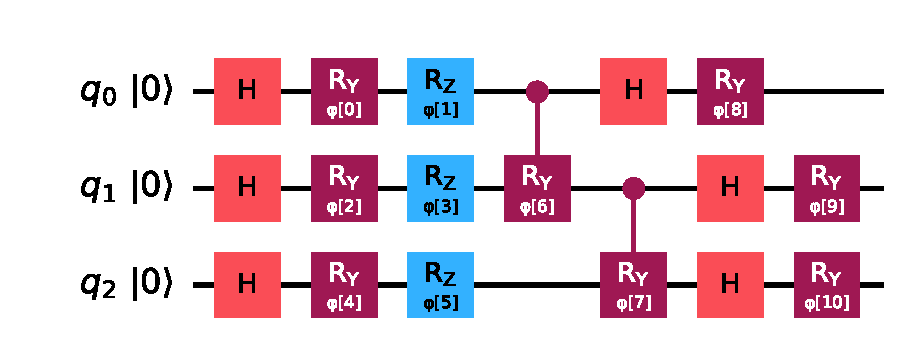
\includegraphics[width=\textwidth]{figs/qmcmc_propuesta.pdf}
\caption{Circuito de propuesta dibujado con $n=3$ qubits y $L=1$ capa para
que la estructura se lea: $H^{\otimes n}$, luego $L$ capas de $R_Y R_Z$ por
qubit más una cadena de CRY, luego otro $H^{\otimes n}$, y una $R_Y$ final
por qubit. \textbf{Tres qubits corresponden a un modelo de tres parámetros}
(wCDM, GEDE). Para $\Lambda$CDM son dos — ver la figura siguiente.}
\end{figure}

\begin{figure}[htbp]
\centering
\makebox[\textwidth][c]{%
  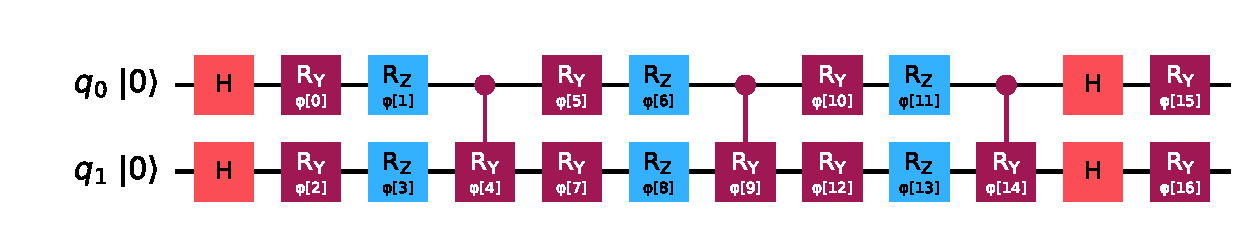
\includegraphics[width=1.1\textwidth]{figs/qmcmc_propuesta_lcdm.pdf}}
\caption{El circuito de propuesta \textbf{tal como corre} para $\Lambda$CDM:
$n=2$ qubits (uno por parámetro: $\Omega_m$ y $H_0$) y $L=3$ capas, que es la
configuración de la campaña. Son $17$ ángulos, todos sorteados al azar en
cada propuesta. Compárese con la figura anterior: misma estructura, distinto
ancho. El ancho lo fija el \emph{modelo}, nunca el número de datos.}
\end{figure}

\paragraph{Qué hace.} Los ángulos $\varphi$ se sortean uniformemente en
$[0,2\pi)$ \emph{en cada propuesta}. El estado resultante es distinto cada
vez. Del vector de amplitudes se toman las primeras $d$ componentes
($d$ = número de parámetros del modelo) y se construye el desplazamiento
\begin{equation}
  \label{eq:desplazamiento}
  \delta_k \;=\; \operatorname{Re}(\psi_k)\cdot
                 \operatorname{sign}\!\big(\operatorname{Im}(\psi_k)\big),
  \qquad k = 1,\dots,d ,
\end{equation}
que se escala por un paso calibrado y se suma al punto actual:
$\theta' = \theta + s\,\delta$.

\paragraph{Por qué produce ese resultado.} Aquí está el punto que importa.
Metropolis \emph{no} exige que la propuesta sea gaussiana. Exige que sea
\textbf{simétrica}: $q(\theta'\mid\theta) = q(\theta\mid\theta')$. Si eso se
cumple, el cociente de Hastings se cancela y la cadena converge a la
posterior correcta sea cual sea la forma de $q$.

Con ángulos uniformes, $\ket{\psi}$ es aproximadamente un vector aleatorio
sobre la esfera unitaria de $\mathbb{C}^{2^n}$. Dos consecuencias:

\begin{enumerate}[leftmargin=1.6em]
  \item Las coordenadas de un vector aleatorio sobre una esfera de dimensión
    alta son aproximadamente gaussianas de media cero. Así que
    $\operatorname{Re}(\psi_k)$ ya tiene la forma que uno querría, sin
    haberlo pedido.
  \item El factor $\operatorname{sign}(\operatorname{Im}\psi_k)$ es un signo
    aleatorio independiente del módulo, y es lo que \textbf{garantiza la
    simetría exacta}: $\delta$ y $-\delta$ tienen la misma probabilidad por
    construcción, no por aproximación.
\end{enumerate}

O sea: el circuito es un generador de números aleatorios con correlaciones
entre coordenadas (las capas CRY las meten), leído de forma que la
distribución resultante sea exactamente simétrica. Es una sustitución
\Cu{algorítmica} legítima: cambia el mecanismo, respeta la condición que el
algoritmo necesita.

\paragraph{Consecuencia para el eje de ruido.} La ecuación
\eqref{eq:desplazamiento} necesita \emph{amplitudes}, y un estado mezclado no
las tiene. Por eso, en cuanto hay ruido, la propuesta debe leerse por la ruta
de cuentas mediante $\langle Z_q\rangle$. Ese cambio de operador es
justamente lo que aísla la columna de control \texttt{none-counts}: ruido
\texttt{none} leído por la ruta de cuentas. Comparar \texttt{none} con
\texttt{readout} sin ese control mezclaría el efecto del ruido con el efecto
de haber cambiado de operador de lectura.

% ---------------------------------------------------------------------
\subsection{Circuito 2 — la aceptación}\label{sec:aceptacion}
\etiqueta{fiel}{FIEL}

\begin{figure}[htbp]
\centering
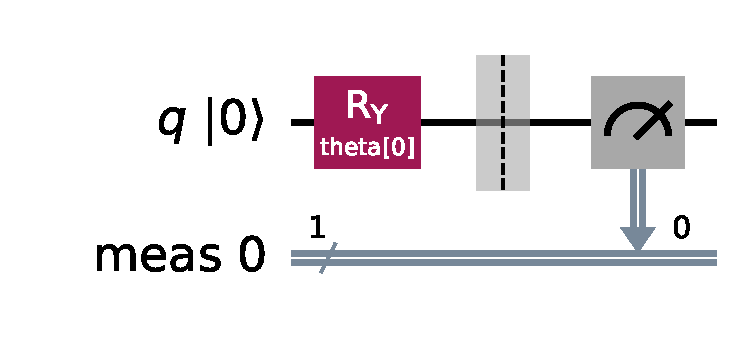
\includegraphics[width=0.30\textwidth]{figs/qmcmc_aceptacion.pdf}
\caption{Circuito de aceptación: un qubit, una rotación, una medición.
El circuito más pequeño del proyecto y el único con una prueba de corrección
exacta.}
\end{figure}

\paragraph{Qué hace.} Sea $\Delta = \log p(\theta') - \log p(\theta)$ y sea
$A = \min(1, e^{\Delta})$ la probabilidad de aceptación de Metropolis. Se
prepara el ángulo
\begin{equation}
  \theta_A \;=\; 2\arccos\!\sqrt{A}
\end{equation}
y se aplica $R_Y(\theta_A)$ a un qubit en $\ket{0}$.

\paragraph{Por qué produce ese resultado.} Por definición de $R_Y$,
\begin{equation}
  R_Y(\theta_A)\ket{0}
  \;=\; \cos\!\frac{\theta_A}{2}\,\ket{0}
      + \sin\!\frac{\theta_A}{2}\,\ket{1},
\end{equation}
y por tanto
\begin{equation}
  \Pr(\text{medir } 0)
  \;=\; \cos^2\!\frac{\theta_A}{2}
  \;=\; \cos^2\!\big(\arccos\sqrt{A}\big)
  \;=\; A .
\end{equation}
Medir el qubit y aceptar si sale $0$ \textbf{es} la regla de Metropolis. No
se parece: es la misma, exactamente. De ahí la etiqueta \Fi{FIEL} y de ahí
que \texttt{QMCMC 50\%} y \texttt{QMCMC 100\%} tengan que coincidir en
todos los dígitos del CSV cuando el peldaño es ideal. En la campaña de
Nicte-Ha esa igualdad se cumple en 72 de 72 celdas comparadas.

\paragraph{Qué le hace el ruido.} Con ruido de lectura, medir $0$ deja de
tener probabilidad $A$ y pasa a tener
$A(1-p) + (1-A)p$ con $p$ la tasa de volteo. La cadena sigue siendo una
cadena de Markov válida, pero de una \emph{distribución estacionaria
distinta} de la posterior. Ese es el sentido físico de que las celdas fieles
ruidosas deban \emph{separarse}: si no se separaran, el modelo de ruido no
estaría entrando.

% =====================================================================
\section{QVMC — variacional sobre una rejilla discreta}
% =====================================================================

El QVMC representa la posterior discretizada en una rejilla de $2^{n_{qpp}}$
puntos por parámetro como $|\psi(\varphi)|^2$, y ajusta los ángulos
$\varphi$ para minimizar
\begin{equation}
  \label{eq:kl}
  \mathrm{KL}(Q_\varphi \,\|\, P)
  \;=\; \sum_x Q_\varphi(x)\,
        \log\frac{Q_\varphi(x)}{P(x)},
  \qquad Q_\varphi(x) = |\psi_x(\varphi)|^2 .
\end{equation}
Tiene \textbf{tres} componentes conmutables, y los tres se apoyan en el mismo
circuito de ansatz. Conviene decirlo explícitamente porque es fuente de
confusión: el circuito 3 se usa en dos de los tres componentes.

% ---------------------------------------------------------------------
\subsection{Circuito 3 — el ansatz (muestreo)}
\etiqueta{cuantico}{ALGORÍTMICO en el entrenamiento, FIEL en el muestreo}

\begin{figure}[htbp]
\centering
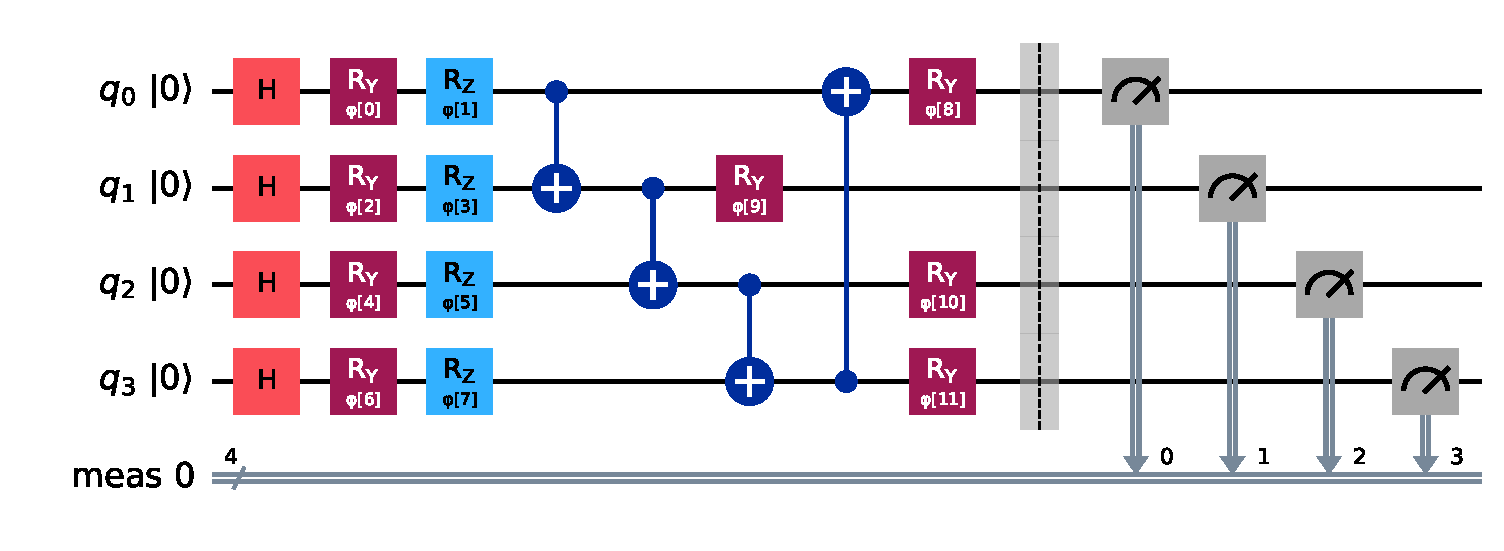
\includegraphics[width=\textwidth]{figs/qvmc_ansatz.pdf}
\caption{Ansatz \emph{hardware-efficient} con $n=4$ qubits y $L=1$ capa; en
la campaña $L=3$. Cada capa: $R_Y R_Z$ por qubit y una cadena de CX cerrada
en anillo. Al final, una $R_Y$ por qubit y la medición.}
\end{figure}

\paragraph{Qué hace.} Con $n$ qubits el circuito cubre $2^n$ cadenas, que
son los $2^n$ puntos de la rejilla. El número de ángulos libres es
\begin{equation}
  n_\varphi \;=\; n\,(2L+1),
\end{equation}
es decir $7n$ con $L=3$.

\paragraph{Por qué produce ese resultado --- y por qué le cuesta.} Los
Hadamard iniciales ponen la misma amplitud en las $2^n$ cadenas. Las
rotaciones $R_Y, R_Z$ mueven amplitud qubit por qubit; los CX en anillo son
los que crean \emph{correlaciones} entre qubits, y sin ellos la distribución
$Q_\varphi$ sería forzosamente un producto de $n$ distribuciones
independientes de un bit --- incapaz de representar cualquier posterior con
covarianza entre parámetros.

Ahora la cuenta que explica por qué la KL nunca baja mucho. La distribución
objetivo sobre $2^n$ puntos tiene $2^n - 1$ grados de libertad. El ansatz
tiene $7n$ ángulos. Con $n=16$ qubits:
\begin{equation}
  2^{16} - 1 = 65\,535 \quad\text{contra}\quad 7\times 16 = 112,
\end{equation}
un déficit de un factor $585$. La familia variacional simplemente no contiene
la distribución objetivo, y el mínimo alcanzable de la KL no es cero: es la
distancia de $P$ a la variedad que el ansatz puede recorrer. En los datos de
la campaña la mejor KL medida es $0.166$, y \emph{empeora} al subir
$n_{qpp}$ (en $\Lambda$CDM va de $0.166$ a $0.447$), exactamente como predice
esta cuenta: cada qubit añadido duplica los grados de libertad del objetivo y
solo añade $7$ ángulos.

Esto no es un defecto de la implementación. Es la limitación estructural de
un ansatz \emph{hardware-efficient}, y conviene reportarla así.

\paragraph{Muestreo: por qué es \Fi{FIEL}.} El componente de muestreo decide
si los puntos se sacan midiendo el circuito o por transformada inversa
clásica sobre el mismo $Q_\varphi$. Las dos rutas muestrean de la misma
distribución, así que en el límite de disparos infinitos coinciden; con
disparos finitos difieren solo por error de Monte Carlo.

% ---------------------------------------------------------------------
\subsection{Circuito 3bis — el gradiente por desplazamiento de parámetro}
\etiqueta{cuantico}{ALGORÍTMICO}

No es un circuito nuevo: es \textbf{el mismo ansatz evaluado en ángulos
desplazados}. Lo menciono aparte porque es el componente de
\emph{entrenamiento} de la escalera y porque es el que cuesta.

Esto explica una cuenta que no cuadra al contar dibujos: el QVMC tiene
\textbf{tres componentes} conmutables (muestreo, entrenamiento,
normalización) pero solo \textbf{dos circuitos distintos}. El entrenamiento
no tiene circuito propio.

\begin{figure}[H]
\centering
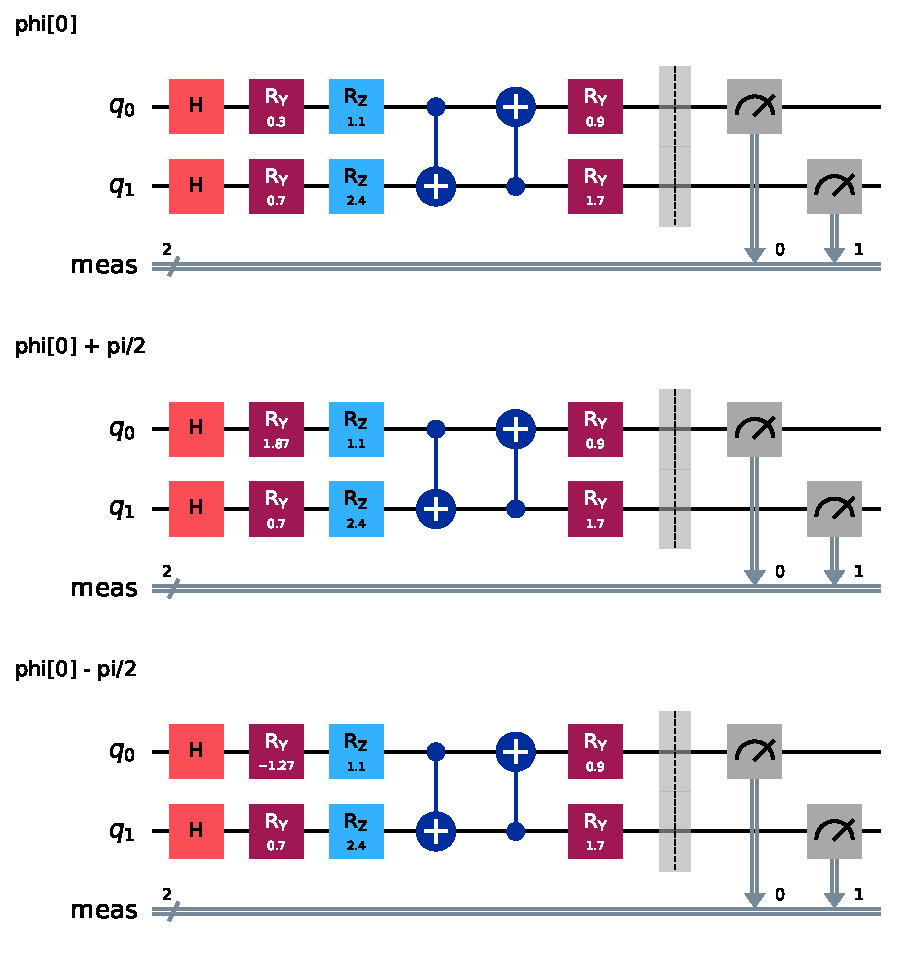
\includegraphics[width=0.82\textwidth]{figs/qvmc_gradiente.pdf}
\caption{El «tercer circuito» del QVMC. Es el mismo ansatz tres veces: la
estructura no cambia, los CX no cambian, y de los seis ángulos solo se mueve
el primero ($0.30 \to 1.87 \to -1.27$, es decir $\varphi_0$,
$\varphi_0+\pi/2$, $\varphi_0-\pi/2$). Se ejecutan los tres, se leen tres
valores de la KL, y la derivada respecto a $\varphi_0$ sale de restarlos.
Para el siguiente ángulo se repite con $\varphi_1$, y así con los
$n_\varphi$.}
\end{figure}

Para una compuerta generada por un operador con valores propios
$\pm\tfrac12$ --- que es el caso de $R_Y$ y $R_Z$ --- se cumple la identidad
\emph{exacta}
\begin{equation}
  \label{eq:shift}
  \frac{\partial f}{\partial \varphi_j}
  \;=\;
  \frac{f(\varphi_j + \tfrac{\pi}{2}) - f(\varphi_j - \tfrac{\pi}{2})}{2}.
\end{equation}
No es una diferencia finita: no hay paso $h$ que elegir ni error de
truncamiento. Es una identidad algebraica que sale de que
$e^{-i\varphi G/2}$ con $G^2 = I$ se puede escribir como
$\cos(\varphi/2)I - i\sin(\varphi/2)G$.

\paragraph{Qué cuesta.} Cada iteración necesita $1 + 2n_\varphi$ circuitos
(uno para el valor, dos por cada ángulo), contra $1$ circuito por evaluación
de COBYLA. Con $n=16$ y $L=3$ eso es $225$ circuitos por iteración. Es la
razón principal de que el peldaño del $100\%$ del QVMC sea el más caro de
toda la campaña.

% ---------------------------------------------------------------------
\subsection{Circuito 4 — la normalización}
\etiqueta{fiel}{FIEL POR CONSTRUCCIÓN}

\begin{figure}[htbp]
\centering
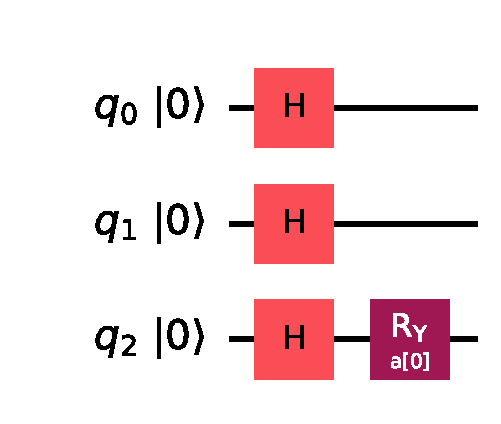
\includegraphics[width=0.34\textwidth]{figs/qvmc_normalizacion.pdf}
\caption{Circuito de normalización tipo QAE con $n=2$ qubits de registro más
un ancila. El ángulo $a$ codifica la suma buscada.}
\end{figure}

\paragraph{Qué hace.} Se preparan $n$ qubits en superposición uniforme y se
rota una ancila con
\begin{equation}
  a \;=\; 2\arcsin\!\sqrt{\frac{\sum_x P_x}{2^{\,n}}},
\end{equation}
de modo que la probabilidad de medir $1$ en la ancila es exactamente
$\big(\sum_x P_x\big)/2^n$. Un estimador de amplitud (QAE) recupera esa
cantidad con error $\mathcal{O}(1/M)$ en vez del $\mathcal{O}(1/\sqrt{M})$
del muestreo clásico, y ahí está la ventaja teórica del componente.

\paragraph{Aviso que hay que declarar en el paper.} En la implementación
actual el circuito \textbf{se ejecuta} bajo el peldaño de ruido activo, pero
\textbf{su resultado se descarta}: la función devuelve la suma exacta
calculada clásicamente. Está documentado así en el código. Dos consecuencias
que no se pueden omitir al leer la escalera:

\begin{enumerate}[leftmargin=1.6em]
  \item El componente es \Fi{fiel} por construcción, no por haberlo
    verificado. La igualdad \texttt{QVMC 67\%} $=$ \texttt{QVMC 100\%} en
    el peldaño ideal es una consecuencia trivial de esto, no una prueba de
    corrección como sí lo es la del QMCMC.
  \item El componente es \textbf{inmune al ruido}. Cualquier degradación
    observada entre el $67\%$ y el $100\%$ viene de otro sitio, y
    atribuirla a la normalización sería un error de lectura.
\end{enumerate}

% =====================================================================
\section{QGA — algoritmo genético con operadores cuánticos}
% =====================================================================

Un algoritmo genético mantiene una población de candidatos y la evoluciona
con tres operadores: cómo se crea la población inicial, cómo muta un
individuo, y cómo se combinan dos padres. El QGA sustituye los tres, uno a
la vez. Cada parámetro se codifica en $n_b$ bits, o sea una rejilla de
$2^{n_b}$ valores por eje.

% ---------------------------------------------------------------------
\subsection{Circuito 5 — la inicialización}
\etiqueta{cuantico}{ALGORÍTMICO}

\begin{figure}[htbp]
\centering
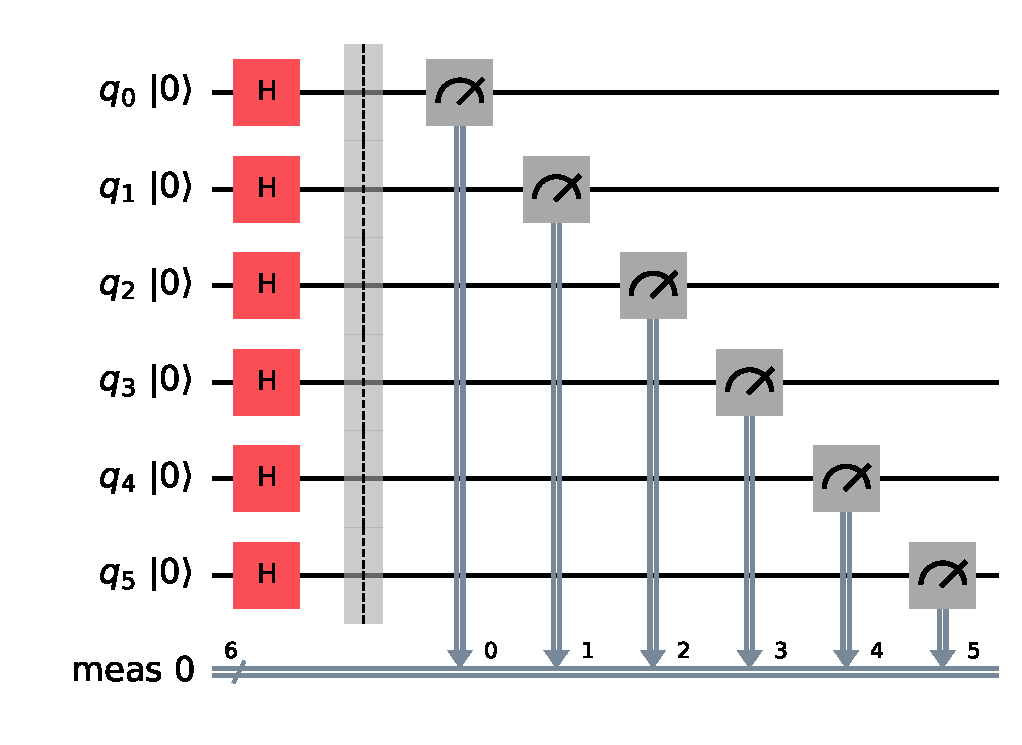
\includegraphics[width=0.62\textwidth]{figs/qga_init.pdf}
\caption{Inicialización con $d=2$ parámetros y $n_b=3$ bits: $d\cdot n_b = 6$
qubits en superposición uniforme, medidos de una vez.}
\end{figure}

\paragraph{Qué hace y por qué.} $H^{\otimes d n_b}$ deja los $2^{d n_b}$
puntos de la rejilla con la misma amplitud, así que una medición devuelve un
punto uniformemente al azar. Un lote de $P$ mediciones es la población
inicial.

Es el circuito más simple del proyecto y es honesto decir lo que es: un
generador de números aleatorios cuántico. No hay interferencia que explotar
--- no hay ninguna compuerta después de los Hadamard --- así que la
distribución es idéntica a la que daría \texttt{numpy}. La sustitución es
\Cu{algorítmica} porque cambia el mecanismo, pero es la que menos puede
cambiar el resultado, y eso se ve en los tiempos: el peldaño del $33\%$
cuesta prácticamente lo mismo que el clásico.

% ---------------------------------------------------------------------
\subsection{Circuito 6 — la mutación}
\etiqueta{cuantico}{ALGORÍTMICO}

\begin{figure}[htbp]
\centering
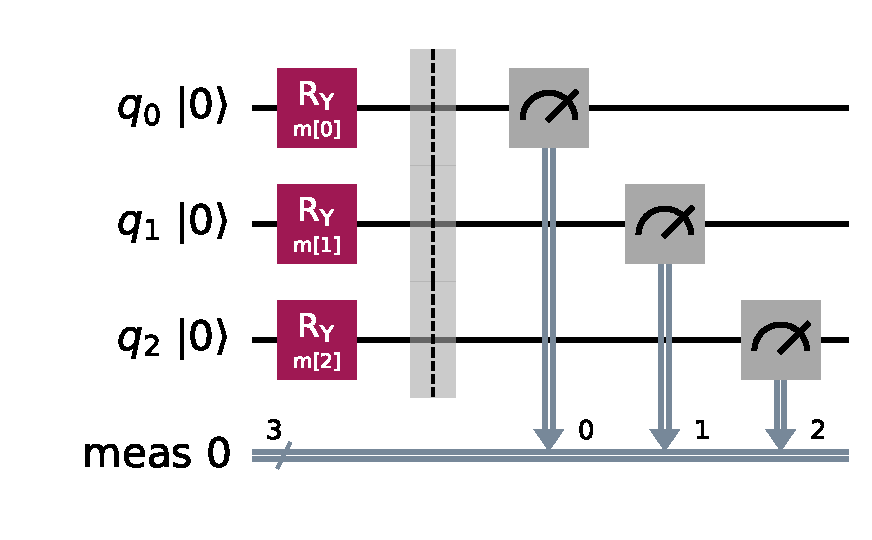
\includegraphics[width=0.40\textwidth]{figs/qga_mutacion.pdf}
\caption{Mutación de un gen de $n_b=3$ bits. Los bits del individuo entran
\emph{en los ángulos}, no como compuertas $X$ estructurales.}
\end{figure}

\paragraph{Qué hace.} Un qubit que representa el bit $b$ con probabilidad de
volteo $p$ debe medir $1$ con probabilidad
\begin{equation}
  P_1 \;=\; b\,(1-p) + (1-b)\,p ,
\end{equation}
y eso se consigue con una sola rotación:
\begin{equation}
  R_Y\big(2\arcsin\sqrt{P_1}\big)\ket{0}
  \quad\Longrightarrow\quad
  \Pr(\text{medir }1) = \sin^2\!\big(\arcsin\sqrt{P_1}\big) = P_1 .
\end{equation}

\paragraph{Por qué está construido así.} Meter el bit en el ángulo, y no
como una compuerta $X$ antes de la rotación, tiene una consecuencia práctica
grande: el circuito es \textbf{el mismo} para todos los individuos, y solo
cambian los ángulos. Eso permite transpilar una única vez y después
\emph{ligar parámetros}, en lugar de transpilar un circuito nuevo por cada
individuo y cada gen. La versión anterior hacía lo segundo
(con $P=200$ y $d=4$, unas $800$ transpilaciones por generación) y eso
dominaba el tiempo de ejecución del QGA.

% ---------------------------------------------------------------------
\subsection{Circuito 7 — el cruce}
\etiqueta{cuantico}{ALGORÍTMICO}

\begin{figure}[htbp]
\centering
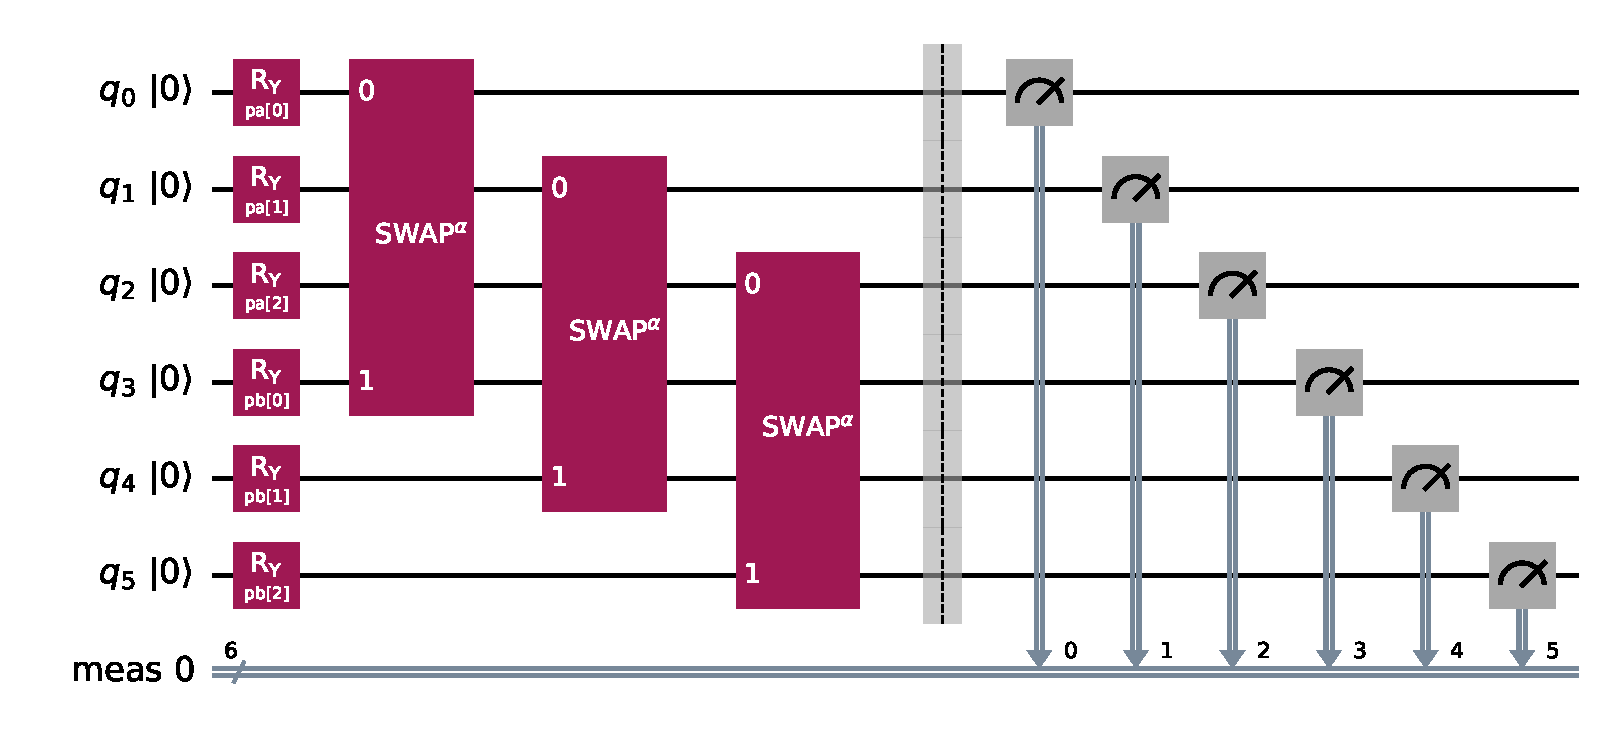
\includegraphics[width=0.78\textwidth]{figs/qga_cruce.pdf}
\caption{Cruce con $n_b=3$: los qubits $q_0..q_2$ llevan al padre A y
$q_3..q_5$ al padre B; un SWAP parcial une cada par de genes homólogos. Es
el único circuito del proyecto con una compuerta de dos qubits arbitraria, y
por eso el único que obliga al transpilador a sintetizar.}
\end{figure}

\paragraph{Qué hace.} Los bits de los dos padres se cargan en ángulos
($R_Y(\pi)\ket{0}=\ket{1}$, $R_Y(0)\ket{0}=\ket{0}$) y sobre cada par de
qubits homólogos se aplica el SWAP parcial
\begin{equation}
  \mathrm{SWAP}^{\alpha}
  \;=\;
  \begin{pmatrix}
    1 & 0 & 0 & 0\\
    0 & \tfrac{1+e^{i\pi\alpha}}{2} & \tfrac{1-e^{i\pi\alpha}}{2} & 0\\
    0 & \tfrac{1-e^{i\pi\alpha}}{2} & \tfrac{1+e^{i\pi\alpha}}{2} & 0\\
    0 & 0 & 0 & 1
  \end{pmatrix}.
\end{equation}
Se mide el registro A y esa es la descendencia.

\paragraph{Por qué produce ese resultado.} Mirando la matriz, el operador es
la identidad sobre $\ket{00}$ y $\ket{11}$, y rota únicamente dentro del
subespacio $\mathrm{span}\{\ket{01},\ket{10}\}$. Tabla de verdad:
\begin{center}
\small
\begin{tabular}{ccl}
\toprule
padres $(a,b)$ & hijo & comentario \\
\midrule
$(0,0)$ & $0$ siempre & consenso preservado \\
$(1,1)$ & $1$ siempre & consenso preservado \\
$a\neq b$ & $a$ con prob.\ $\cos^2(\pi\alpha/2)$, si no $b$ & herencia por interferencia \\
\bottomrule
\end{tabular}
\end{center}
Con $\alpha=1/2$ eso es el análogo cuántico de un cruce \emph{uniforme} bit a
bit (50/50); $\alpha\to0$ conserva al padre A y $\alpha\to1$ trae al B. Las
amplitudes $(1\pm e^{i\pi\alpha})/2$ son complejas: hay interferencia real
entre los bits en desacuerdo, no una moneda clásica disfrazada.

\paragraph{Por qué no es la versión obvia.} La implementación anterior usaba
CX seguido de CRY, cuya tabla de verdad medida era
$\{(0,0)\to0,\ (0,1)\to0.85,\ (1,0)\to1,\ (1,1)\to0.146\}$: el hijo era
aproximadamente $a \oplus b$. Mapear $(1,1)\to0$ con probabilidad $0.85$
destruye exactamente los bits en los que una población convergida está de
acuerdo, que es lo contrario de lo que un cruce debe hacer.

\paragraph{Por qué es el circuito caro.} Usa $2n_b$ qubits --- el doble que
los otros dos operadores. Con ruido el simulador pasa a matriz de densidad,
que es $2^{2n_b}\times 2^{2n_b}$ en vez de un vector de $2^{2n_b}$. Medido en
la campaña de Nicte-Ha, para $\Lambda$CDM:

\begin{center}
\small
\begin{tabular}{lrrr}
\toprule
$n_b$ & \texttt{none} & \texttt{readout} & \texttt{full} \\
\midrule
4 & 125\,s   & 1\,489\,s   & --- \\
5 & 181\,s   & 22\,035\,s  & 21\,544\,s \\
6 & 202\,s   & 327\,281\,s & 334\,682\,s \\
7 & 405\,s   & no terminó  & no terminó \\
\bottomrule
\end{tabular}
\end{center}

\noindent
A $n_b=6$ el ruido cuesta un factor $\sim 1\,600$. Los peldaños del $0$,
$33$ y $67\%$ no lo notan porque sus circuitos son de $n_b$ qubits, no de
$2n_b$.

% =====================================================================
\clearpage
% =====================================================================
\section{Qué entra y qué sale: una traza con números reales}
% =====================================================================

Un diagrama de circuito no enseña lo que más cuesta ver: dónde termina lo
clásico, qué objeto cruza la frontera, y cómo vuelve a ser un número. Esta
sección traza \emph{un} paso de cada algoritmo sobre el posterior real
($\Lambda$CDM, CC+BAO+Pantheon, $1\,099$ datos) e imprime cada cruce.

Los números de abajo no están inventados: salen de ejecutar
\texttt{docs/circuitos/traza\_un\_paso.py}, que corre sobre el mismo código
de la campaña. La traza completa se regenera con

\begin{center}
\texttt{python docs/circuitos/traza\_un\_paso.py}
\end{center}

% ---------------------------------------------------------------------
\subsection{QMCMC: un paso de Metropolis, de principio a fin}

\begin{center}
\small
\begin{tabular}{@{}llll@{}}
\toprule
& \textbf{Qué cruza} & \textbf{Tipo} & \textbf{Valor} \\
\midrule
\multicolumn{4}{@{}l}{\Cl{1. CLÁSICO} — el punto actual} \\
& $\theta$              & \texttt{float[2]}  & $(0.2800,\; 69.500)$ \\
& $\log p(\theta)$      & \texttt{float}     & $-532.3972$ \;\; \emph{aquí entran los 1\,099 datos} \\
\addlinespace
\multicolumn{4}{@{}l}{\Cu{2. CUÁNTICO} — la propuesta} \\
& ancho del circuito    & \texttt{int}       & $2$ qubits \;(= $d$, \textbf{no} $n_{\text{datos}}$) \\
& ángulos de entrada    & \texttt{float[17]} & sorteados en $[0,2\pi)$ — \textbf{nada} del problema \\
& lo que sale de Aer    & \texttt{complex[4]}& el vector de estado completo \\
& $\mathrm{Re}(\psi)\,\mathrm{sign}(\mathrm{Im}\,\psi)$ & \texttt{float[2]} & $(-0.0756,\; -0.4438)$ \\
& $\theta' = \theta + s\delta$ & \texttt{float[2]} & $(0.2762,\; 67.281)$ \\
\addlinespace
\multicolumn{4}{@{}l}{\Cl{3. CLÁSICO} — evaluar el propuesto} \\
& $\log p(\theta')$     & \texttt{float}     & $-542.7681$ \;\; \emph{otra vez los 1\,099 datos} \\
& $\Delta$              & \texttt{float}     & $-10.3709$ \\
& $A = \min(1,e^{\Delta})$ & \texttt{float}  & $0.000031$ \\
\addlinespace
\multicolumn{4}{@{}l}{\Fi{4. CUÁNTICO} — la aceptación (1 qubit)} \\
& ángulo de entrada     & \texttt{float}     & $\theta_A = 3.130398$ rad \;\; \textbf{un solo número} \\
& lo que sale           & \texttt{float}     & $\Pr(\text{medir }0) = 0.000031$ \\
& comprobación          & ---                & $|\Pr(0) - A| = 1\times10^{-12}$ \\
& decisión              & \texttt{bool}      & $u = 0.5 > \Pr(0)$ $\Rightarrow$ \textbf{rechaza} \\
\bottomrule
\end{tabular}
\end{center}

\noindent
Lo que hay que ver en esa tabla: los $1\,099$ datos entraron \textbf{dos
veces}, las dos de forma clásica, y de todo ese cálculo sobrevivió
\textbf{un solo número} ($A$) hasta tocar un qubit. El circuito de propuesta
ni siquiera vio el problema: se le dan $17$ ángulos aleatorios y devuelve un
desplazamiento. El de aceptación recibe un número y devuelve una moneda
cargada con ese número.

\paragraph{Cómo se convierte el circuito en número, exactamente.} En el paso
2 el simulador entrega las cuatro amplitudes $\psi_0,\dots,\psi_3$ y la regla
de lectura toma las dos primeras. En el paso 4 el simulador entrega
$\Pr(0)=|\psi_0|^2$ directamente. \textbf{Ése es todo el puente}: una regla
fija que convierte amplitudes (o frecuencias de medición) en los números que
el algoritmo clásico necesita. Cambiar esa regla es cambiar el algoritmo, y
por eso el eje de ruido tiene que declarar cuál usa (sección 1).

% ---------------------------------------------------------------------
\subsection{QVMC: una evaluación de la KL}

\begin{center}
\small
\begin{tabular}{@{}llll@{}}
\toprule
& \textbf{Qué cruza} & \textbf{Tipo} & \textbf{Valor} \\
\midrule
\multicolumn{4}{@{}l}{\Cl{1. CLÁSICO} — la rejilla y el objetivo} \\
& ancho del circuito & \texttt{int} & $6$ qubits $= d(2)\times n_{qpp}(3)$ \\
& puntos de rejilla  & \texttt{int} & $2^6 = 64$ \\
& $P$ (objetivo)     & \texttt{float[64]} & $\sum P = 1$ \;\; \emph{construido con los 1\,099 datos} \\
& \texttt{theta\_table} & \texttt{float[64,2]} & cadena de bits $\to$ punto de parámetros \\
\addlinespace
\multicolumn{4}{@{}l}{\Cu{2. CUÁNTICO} — el ansatz} \\
& ángulos de entrada & \texttt{float[18]} & $n_\varphi = n(2L+1) = 6\cdot 3$ \\
& lo que sale de Aer & \texttt{float[64]} & $|\psi_x|^2$, con $\sum = 1.0000000000$ \\
& $Q$                & \texttt{float[64]} & máx $= 0.0617$ en la celda $21$ \\
\addlinespace
\multicolumn{4}{@{}l}{\Cl{3. CLÁSICO} — comparar $Q$ contra $P$} \\
& $\mathrm{KL}(Q\|P)$ & \texttt{float} & $19.4930$ \;\; \textbf{un número} \\
& estimador $E_Q[\theta]$ & \texttt{float[2]} & $(0.3298,\; 71.437)$ \\
\bottomrule
\end{tabular}
\end{center}

\noindent
(La KL sale alta porque la traza usa $\varphi_j = 0.3$ para todos, o sea el
ansatz \emph{sin entrenar}. Entrenado baja a los valores de la campaña.)

El circuito \textbf{nunca vio los datos}: produjo $Q$. Los datos vivían en
$P$. Las dos distribuciones se comparan clásicamente y de ahí sale el único
número que el optimizador intenta bajar.

\paragraph{Y aquí se ve por qué son tres componentes con dos dibujos.}
Siguiendo la traza, el mismo circuito con $\varphi_0$ corrido:

\begin{center}
\small
\begin{tabular}{@{}lll@{}}
\toprule
mismo circuito, $\varphi_0 + \pi/2$ & KL & $18.1772$ \\
mismo circuito, $\varphi_0 - \pi/2$ & KL & $19.3555$ \\
\midrule
$\partial\,\mathrm{KL}/\partial\varphi_0$ & derivada \textbf{exacta}
  & $(18.1772 - 19.3555)/2 = -0.5892$ \\
costo de una iteración & circuitos & $1 + 2\cdot 18 = 37$ \\
\bottomrule
\end{tabular}
\end{center}

\noindent
Tres ejecuciones del \emph{mismo} circuito con un ángulo distinto dan una
derivada exacta. Repetido para los $18$ ángulos, son $37$ circuitos por
iteración. Ésa es toda la diferencia entre el peldaño del $33\%$ y el del
$67\%$ del QVMC, y explica el salto de costo.

% ---------------------------------------------------------------------
\subsection{QGA: un gen mutado}

\begin{center}
\small
\begin{tabular}{@{}llll@{}}
\toprule
& \textbf{Qué cruza} & \textbf{Tipo} & \textbf{Valor} \\
\midrule
\multicolumn{4}{@{}l}{\Cl{1. CLÁSICO} — el individuo, como bits} \\
& $\theta$ (un individuo) & \texttt{float[2]} & $(0.2800,\; 69.500)$ \\
& genes (enteros)         & \texttt{int[2]}   & $(2,\;3)$ en una rejilla de $2^3$ \\
& bits                    & \texttt{int[2,3]} & \texttt{010}\;\;\texttt{011} \\
\addlinespace
\multicolumn{4}{@{}l}{\Cu{2. CUÁNTICO} — la mutación} \\
& ancho del circuito & \texttt{int} & $3$ qubits $= n_b$ \\
& $P_1 = b(1-p)+(1-b)p$ & \texttt{float[3]} & $(0.2,\;0.8,\;0.2)$ con $p=0.2$ \\
& ángulos de entrada & \texttt{float[3]} & $(0.9273,\; 2.2143,\; 0.9273)$ \\
& lo que sale        & bits medidos      & una cadena por disparo: \emph{ése es el gen} \\
\addlinespace
\multicolumn{4}{@{}l}{\Cl{3. CLÁSICO} — decodificar y evaluar} \\
& $\theta$ decodificado & \texttt{float[2]} & $(0.2800,\; 69.625)$ \\
& fitness $\chi^2$      & \texttt{float}    & $1064.976$ sobre $1\,099$ datos \\
\bottomrule
\end{tabular}
\end{center}

\noindent
El circuito solo movió bits. Qué tan bueno es el individuo lo decide el
$\chi^2$, que es clásico de principio a fin.

\medskip
\noindent
\textbf{El patrón, en los tres casos, es el mismo:}

\begin{center}
\small
\begin{tabular}{@{}lll@{}}
\toprule
& \textbf{Entra al circuito} & \textbf{Sale del circuito} \\
\midrule
QMCMC propuesta   & ángulos aleatorios             & amplitudes $\to$ un desplazamiento \\
QMCMC aceptación  & un ángulo (de $A$)             & $\Pr(0) \to$ aceptar o no \\
QVMC ansatz       & los $\varphi$ variacionales    & $|\psi|^2 \to$ la distribución $Q$ \\
QVMC gradiente    & los mismos $\varphi \pm \pi/2$ & tres KL $\to$ una derivada \\
QGA mutación      & ángulos (de los bits)          & bits medidos $\to$ el gen nuevo \\
QGA cruce         & ángulos (de dos padres)        & bits medidos $\to$ el hijo \\
\bottomrule
\end{tabular}
\end{center}

\noindent
Nunca entra un dato. Nunca sale un dato. Entran ángulos, salen amplitudes o
frecuencias, y una regla de lectura fija las convierte en el número que el
algoritmo clásico estaba esperando.

\clearpage
\section{Diagrama de flujo: qué puede ser cuántico}
% =====================================================================

\begin{figure}[H]
\centering
\begin{tikzpicture}[
  font=\small,
  nodo/.style={draw,rounded corners=2pt,align=center,inner sep=5pt,
               minimum height=8mm,text width=30mm,line width=.5pt},
  cl/.style={nodo,draw=clasico,fill=clasico!8},
  qu/.style={nodo,draw=cuantico,fill=cuantico!10,line width=.9pt},
  fi/.style={nodo,draw=fiel,fill=fiel!10,line width=.9pt},
  fl/.style={-{Stealth[length=4pt]},draw=gris,line width=.6pt},
  tit/.style={font=\bfseries\small,text=azulq},
]

% ---- QMCMC ----
\node[tit] (t1) at (0,0) {QMCMC};
\node[cl,below=4mm of t1]        (a1) {punto actual $\theta$};
\node[qu,below=4mm of a1]        (a2) {\textbf{propuesta}\\[-1pt]{\scriptsize circuito 1 — algorítmico}};
\node[cl,below=4mm of a2]        (a3) {evaluar\\$\log p(\theta')$};
\node[fi,below=4mm of a3]        (a4) {\textbf{aceptación}\\[-1pt]{\scriptsize circuito 2 — fiel}};
\node[cl,below=4mm of a4]        (a5) {cadena};
\foreach \i/\j in {a1/a2,a2/a3,a3/a4,a4/a5} \draw[fl] (\i) -- (\j);
\draw[fl] (a5.west) -- ++(-.7,0) |- (a1.west);

% ---- QVMC ----
\node[tit] (t2) at (5.6,0) {QVMC};
\node[cl,below=4mm of t2]        (b1) {rejilla $2^{n}$\\y objetivo $P$};
\node[qu,below=4mm of b1]        (b2) {\textbf{ansatz} $\ket{\psi(\varphi)}$\\[-1pt]{\scriptsize circuito 3}};
\node[qu,below=4mm of b2]        (b3) {\textbf{gradiente}\\[-1pt]{\scriptsize circuito 3bis — algorítmico}};
\node[fi,below=4mm of b3]        (b4) {\textbf{normalización}\\[-1pt]{\scriptsize circuito 4 — fiel}};
\node[cl,below=4mm of b4]        (b5) {KL final,\\estimador};
\foreach \i/\j in {b1/b2,b2/b3,b3/b4,b4/b5} \draw[fl] (\i) -- (\j);
\draw[fl] (b4.east) -- ++(.7,0) |- (b2.east);

% ---- QGA ----
\node[tit] (t3) at (11.2,0) {QGA};
\node[qu,below=4mm of t3]        (c1) {\textbf{inicialización}\\[-1pt]{\scriptsize circuito 5}};
\node[cl,below=4mm of c1]        (c2) {evaluar $\chi^2$\\y seleccionar};
\node[qu,below=4mm of c2]        (c3) {\textbf{cruce}\\[-1pt]{\scriptsize circuito 7}};
\node[qu,below=4mm of c3]        (c4) {\textbf{mutación}\\[-1pt]{\scriptsize circuito 6}};
\node[cl,below=4mm of c4]        (c5) {mejor de la\\rejilla + refinador};
\foreach \i/\j in {c1/c2,c2/c3,c3/c4,c4/c5} \draw[fl] (\i) -- (\j);
\draw[fl] (c4.east) -- ++(.7,0) |- (c2.east);

% ---- leyenda ----
\node[qu,text width=26mm,anchor=north west] at (-1.2,-9.4) {sustituible\\por cuántico};
\node[fi,text width=26mm,anchor=north west] at (2.6,-9.4)  {fiel: debe\\reproducir al clásico};
\node[cl,text width=26mm,anchor=north west] at (6.4,-9.4)  {clásico siempre\\(la física)};
\end{tikzpicture}
\caption{Los tres algoritmos y los puntos de sustitución. Lo que nunca se
vuelve cuántico es la evaluación de la verosimilitud: calcular $H(z)$,
integrar la distancia lumínica y comparar contra los datos es un cálculo
clásico, y es donde se va casi todo el tiempo de una corrida real.}
\end{figure}

\paragraph{Lectura del diagrama.} Los tres algoritmos comparten una
estructura: hay un lazo, y dentro del lazo hay un punto donde se propone o
se genera un candidato, y otro donde se decide qué hacer con él. Lo cuántico
entra en el \emph{cómo se genera} y en el \emph{cómo se decide}, nunca en el
\emph{cuánto vale}. La cosmología --- la integral de $H(z)$, el módulo de
distancia, el $\chi^2$ contra 1\,099 puntos --- es clásica de principio a
fin, en las tres columnas y en todos los peldaños.

\clearpage
% =====================================================================
\section{Cómo se leen las figuras del eje de ruido}
% =====================================================================

Las figuras que produce \texttt{graficas\_ruido.py} contestan una sola
pregunta: \emph{¿cuánto mueve el ruido al resultado, y ese movimiento crece o
no con el tamaño del registro?} Esta sección explica qué hay en cada eje,
porque los cinco ejes verticales miden cosas distintas y no se leen igual.

% ---------------------------------------------------------------------
\subsection{Las tres familias de figura}

\begin{description}[leftmargin=1.6em,style=nextline]
  \item[Tipo 1 y 2 --- \texttt{ruido\_vs\_rejilla\_*}.]
    Eje $x$: \texttt{nqpp} (samplers) o \texttt{n\_bits} (genético). Un panel
    por peldaño de la escalera, una curva por peldaño de ruido. Contesta:
    \emph{¿el efecto del ruido empeora al agrandar el registro?} Una curva
    que se separa de la azul al avanzar hacia la derecha es una señal de
    alarma; curvas paralelas significan que el ruido cuesta lo mismo sin
    importar el tamaño.
  \item[Tipo 3 --- \texttt{ruido\_fijo\_*}.]
    Eje $x$: los peldaños de la escalera (CGA, QGA 33\%, …). Barras
    agrupadas, una por peldaño de ruido, un panel por métrica. Contesta:
    \emph{a tamaño de registro fijo, ¿cuál de mis métodos aguanta mejor el
    ruido?} Aquí el tamaño del registro no se mete de por medio.
\end{description}

\paragraph{Convenciones de color y trazo.} No son decorativas:

\begin{itemize}[leftmargin=1.6em]
  \item \texttt{none} y \texttt{none-counts} comparten \textbf{el mismo
    color} y se distinguen por el trazo (línea discontinua, barra rayada).
    Es a propósito: son el \emph{mismo} nivel de ruido leído por dos rutas
    distintas, no dos niveles. Darles colores distintos sugeriría una
    gradación que no existe.
  \item \texttt{readout} y \texttt{full} sí son peldaños de la escala y
    llevan color propio.
  \item Los backends reales (\texttt{FakeBrisbane}) usan un color de reserva
    y trazo punto-raya, porque no son peldaños sintéticos y no tienen un
    lugar fijo en la escala.
  \item \textbf{Una curva o barra ausente significa que esa celda no tiene
    dato} --- no corrió, o sigue corriendo --- \emph{no} que valga cero.
\end{itemize}

% ---------------------------------------------------------------------
\subsection{Los cinco ejes $y$, uno por uno}

\subsubsection*{(a) \texttt{desplazamiento} --- el eje que importa}

Es el único que mide si el ruido movió la \emph{física}. Su definición:
\begin{equation}
  \label{eq:desp}
  D \;=\; \max_{k}\;
  \frac{\big|\,p_k(\text{ruido}) - p_k(\text{ideal})\,\big|}
       {\sigma_k(\text{ideal})},
\end{equation}
donde $k$ recorre los parámetros del modelo y la referencia es la corrida
\texttt{none} de la \textbf{misma celda}: mismo modelo, mismo peldaño de la
escalera, mismo \texttt{nqpp}.

\medskip
\noindent
Tres decisiones de diseño que hay que poder defender:

\begin{description}[leftmargin=1.6em,style=nextline]
  \item[Por qué es adimensional.] Dividir entre $\sigma$ convierte
    ``$\Omega_m$ se movió $0.0003$'' --- un número que no dice nada por sí
    solo --- en ``se movió una fracción de tu propia barra de error''.
    Así $\Omega_m$ y $H_0$, que viven en escalas totalmente distintas, caben
    en el mismo eje.
  \item[Por qué el divisor es $\sigma$ de la corrida \emph{ideal}.] Porque el
    ruido tiende a \emph{ensanchar} la posterior. Si se dividiera entre la
    $\sigma$ ruidosa, un sesgo grande acompañado de una posterior ancha daría
    un número pequeño, y el sesgo quedaría escondido detrás de su propia
    dispersión. Con la $\sigma$ ideal en el denominador eso no puede pasar.
  \item[Por qué el máximo y no el promedio.] Si el ruido sesga aunque sea un
    parámetro, el resultado ya está sesgado. Promediar sobre parámetros
    diluiría un sesgo real en $w_a$ con tres parámetros limpios.
\end{description}

\medskip
\noindent
\textbf{Cómo leer el número:}

\begin{center}
\small
\begin{tabular}{ll}
\toprule
$D \approx 0$   & el ruido no movió nada; el resultado es el mismo \\
$D = 0.1$       & se movió una décima de la barra de error: irrelevante \\
$D = 1$         & el sesgo del ruido es tan grande como tu error estadístico \\
$D > 1$         & el ruido domina; el número reportado ya no es el de la posterior \\
\bottomrule
\end{tabular}
\end{center}

\noindent
Por eso las figuras llevan una \textbf{línea punteada horizontal en $1$}: es
el umbral donde el ruido empieza a competir con tu incertidumbre.

\paragraph{Lo medido.} Sobre las dos campañas completas (Nicte-Ha
\texttt{hpc\_20260907\_130425} y Saptiva \texttt{hpc\_20260907\_182345}),
$607$ celdas ruidosas comparables contra su corrida ideal:

\begin{center}
\small
\begin{tabular}{lr}
\toprule
mediana de $D$              & $0.0008\,\sigma$ \\
percentil 90                & $0.14\,\sigma$ \\
celdas con $D > 0.5\,\sigma$ & $11$ \;(1.8\%) \\
celdas con $D > 1\,\sigma$   & $10$ \;(1.6\%) \\
celdas con $D > 2\,\sigma$   & $0$ \\
máximo                      & $1.24\,\sigma$ \\
\bottomrule
\end{tabular}
\end{center}

\noindent
O sea: \textbf{en el $98\%$ de las celdas el ruido deja la cosmología donde
estaba}, pero hay una \emph{cola}, y la cola tiene estructura. Las diez
celdas que cruzan $1\sigma$ son las mismas cinco configuraciones repetidas en
las dos máquinas:

\begin{center}
\small
\begin{tabular}{llll}
\toprule
$D$ & peldaño & celda & método \\
\midrule
$1.24\,\sigma$ & \texttt{full}         & PEDE, $n_{qpp}=4$ & QVMC 67\% y 100\% \\
$1.23\,\sigma$ & \texttt{FakeBrisbane} & PEDE, $n_{qpp}=4$ & QVMC 67\% y 100\% \\
$1.12\,\sigma$ & \texttt{full}         & GEDE, $n_b=4$     & QGA 100\% \\
$1.11\,\sigma$ & \texttt{FakeBrisbane} & LCDM, $n_{qpp}=4$ & QVMC 67\% y 100\% \\
\bottomrule
\end{tabular}
\end{center}

\noindent
Que se reproduzca en dos máquinas independientes es lo que la convierte en un
resultado y no en ruido de una corrida. Tres cosas que conviene decir al
reportarla:

\begin{itemize}[leftmargin=1.6em]
  \item \texttt{readout} \textbf{nunca} cruza: su máximo sobre las $607$
    celdas es $0.39\,\sigma$. El error de lectura solo no sesga.
  \item \texttt{none-counts} tampoco: máximo $0.12\,\sigma$. Cambiar de ruta
    de lectura, por sí mismo, no mueve el resultado --- que es exactamente
    para lo que existe ese control.
  \item La cola es de los peldaños \emph{más} ruidosos (\texttt{full},
    \texttt{FakeBrisbane}), en la rejilla \emph{más} gruesa ($4$ bits o
    qubits por parámetro), y en los modelos con el ajuste más pobre (PEDE
    tiene el $\chi^2_{\mathrm{red}}$ más alto de los cinco). Es la
    combinación donde menos margen hay, y es donde el sesgo aparece primero.
\end{itemize}

\begin{figure}[H]
\centering
\makebox[\textwidth][c]{%
  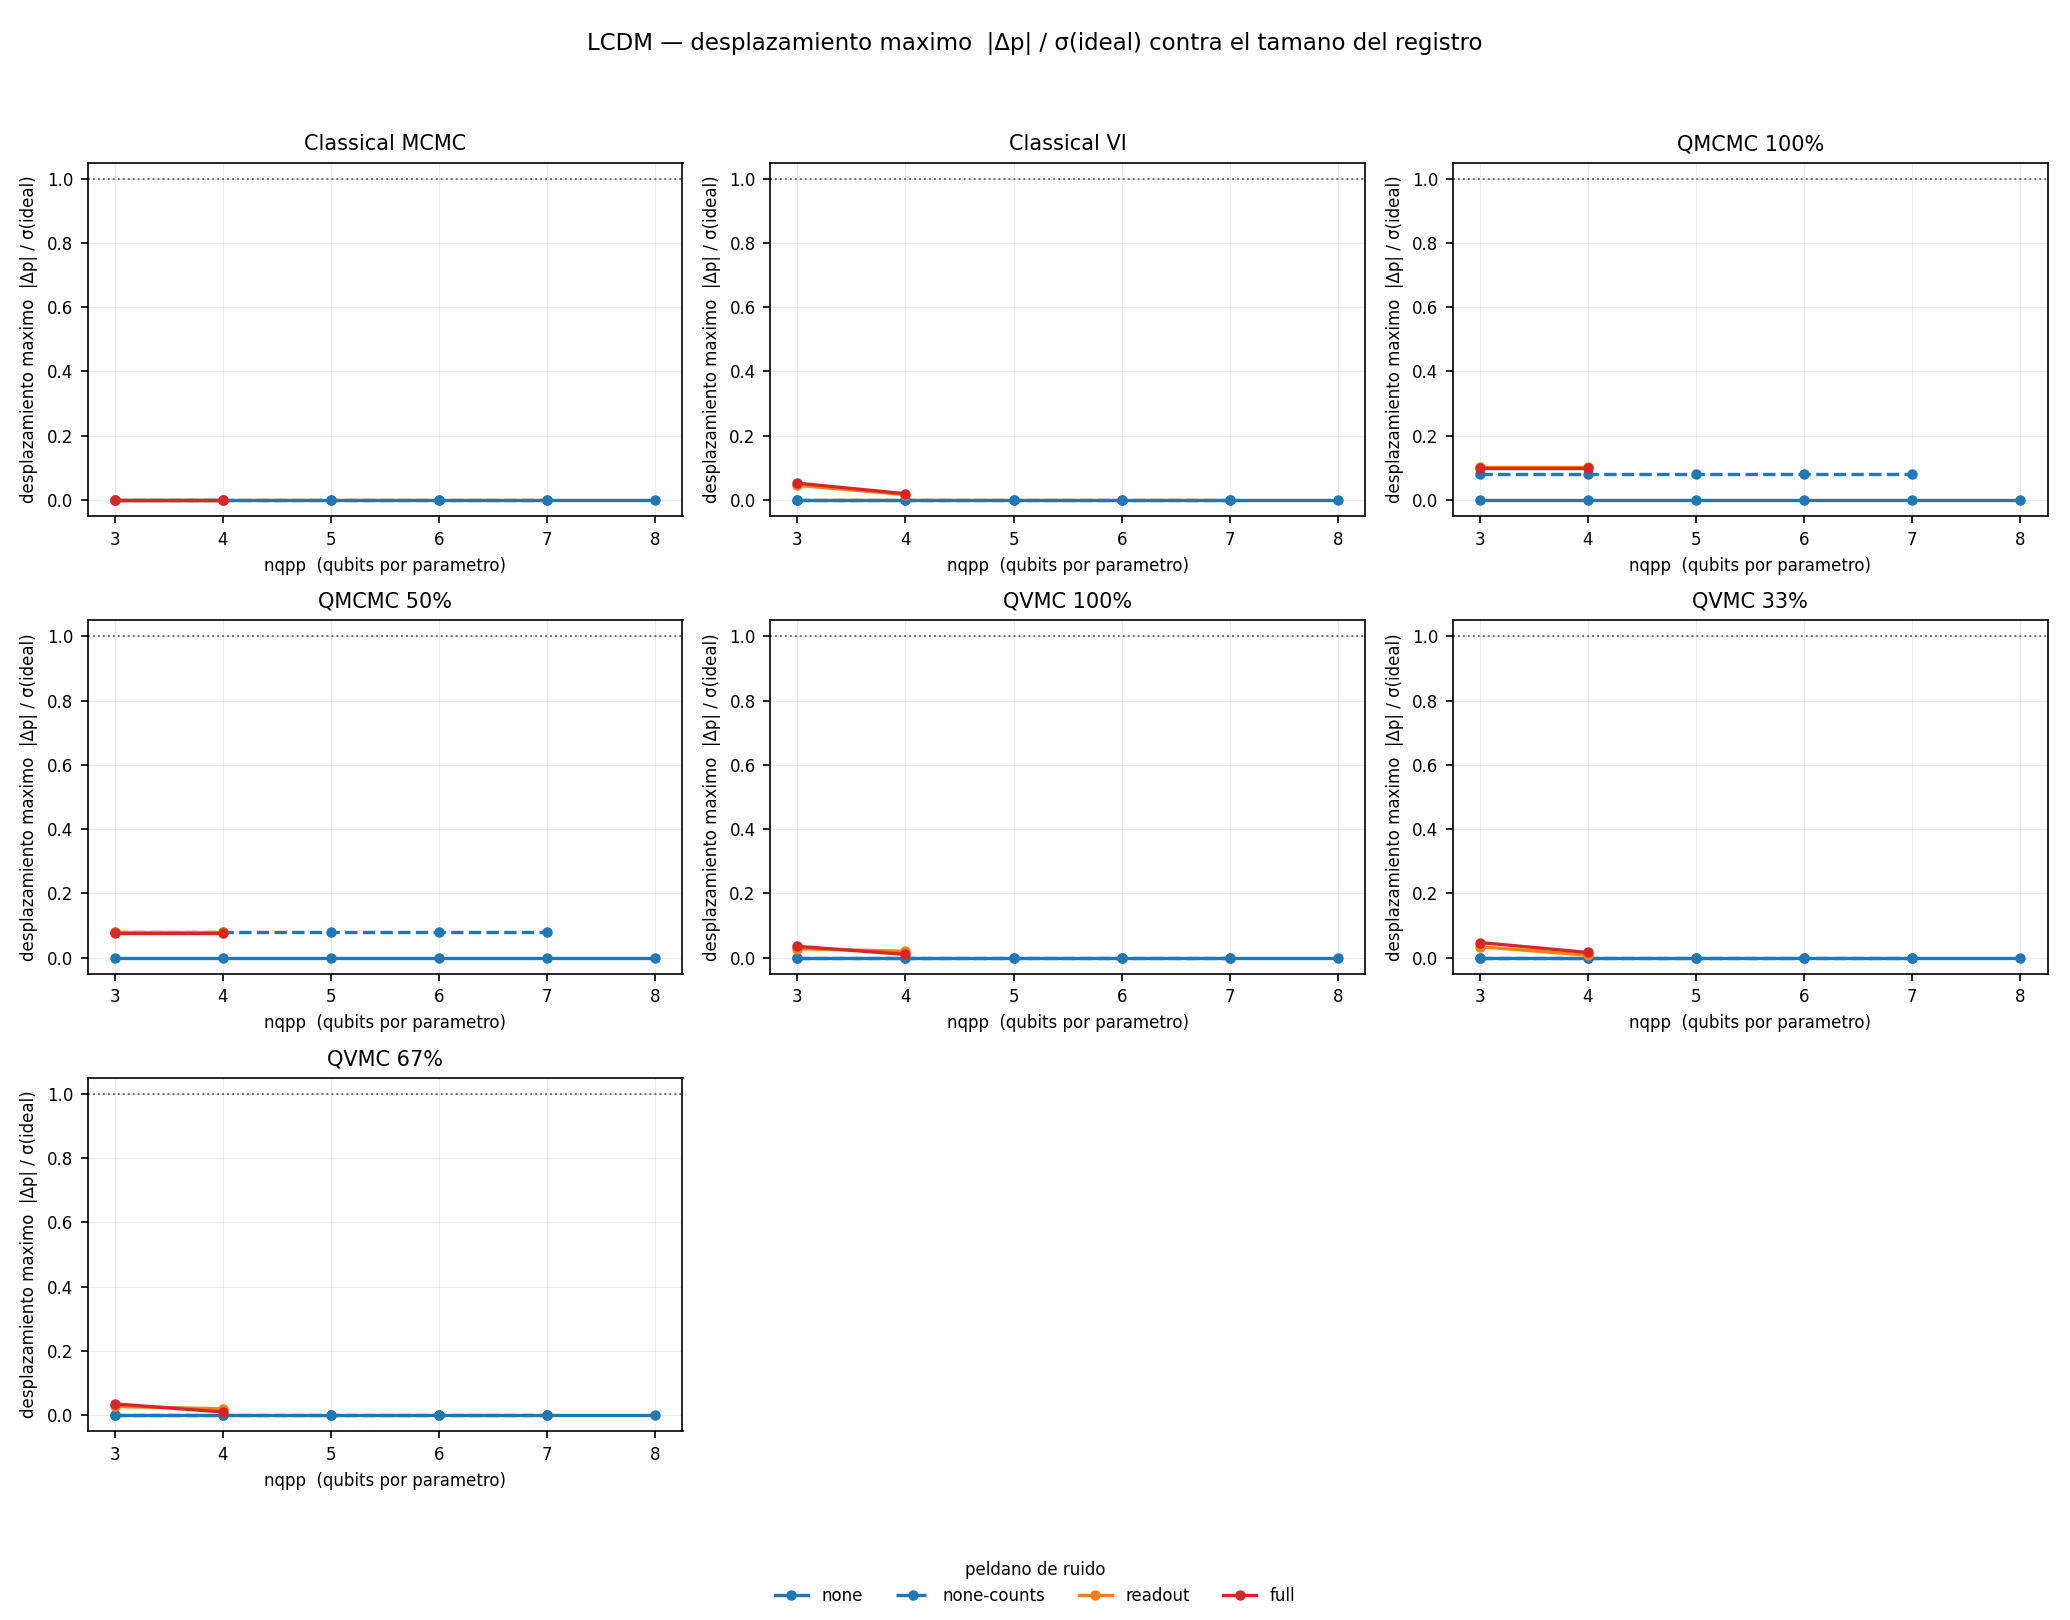
\includegraphics[width=1.22\textwidth]{figs/ejemplo_ruido_vs_rejilla.png}}
\caption{Figura tipo 1: \texttt{desplazamiento} contra \texttt{nqpp} para
$\Lambda$CDM. Un panel por peldaño de la escalera. En este modelo todas las
curvas viven pegadas al cero y la línea de $1\sigma$ queda muy arriba --- es
el caso típico, el del $98\%$ de las celdas. La cola de la tabla anterior
no aparece aquí: está en PEDE y GEDE, no en $\Lambda$CDM. Las curvas naranja
y roja solo llegan a \texttt{nqpp}$=4$ porque los peldaños ruidosos solo se
corrieron hasta ahí.}
\end{figure}

\subsubsection*{(b) \texttt{acceptance} --- salud de la cadena}

Fracción de propuestas aceptadas por Metropolis, entre $0$ y $1$. No es una
medida de calidad del resultado sino de si la cadena se está moviendo:

\begin{itemize}[leftmargin=1.6em]
  \item cerca de $0$: la cadena se atora, casi todo se rechaza;
  \item cerca de $1$: acepta casi todo, o sea el paso es demasiado corto y
    la cadena apenas explora;
  \item una zona sana está más o menos entre $0.2$ y $0.5$.
\end{itemize}

\noindent
Solo la llenan QMCMC y el MCMC clásico; el variacional y el genético dejan la
columna vacía y por eso sus barras no aparecen en ese panel. Medido a
\texttt{nqpp}$=4$: $0.4873$ en los cuatro peldaños de ruido, idéntico a
cuatro decimales. Es un control limpio.

\subsubsection*{(c) \texttt{final\_KL} --- qué tan lejos quedó el variacional}

La divergencia de Kullback--Leibler de la ecuación \eqref{eq:kl}, en nats.
Mide la distancia entre la distribución que el circuito logró producir,
$Q_\varphi$, y la posterior objetivo $P$.

\begin{itemize}[leftmargin=1.6em]
  \item $0$ significa que $Q_\varphi$ reproduce $P$ exactamente. \textbf{No
    se alcanza nunca}, y la sección 4.1 explica por qué: $7n$ ángulos contra
    $2^n-1$ grados de libertad.
  \item No tiene cota superior. Un valor de $2$ no es ``el doble de malo''
    que $1$ en ningún sentido intuitivo; es simplemente más lejos.
  \item \textbf{El eje va en escala logarítmica}, porque en una misma figura
    conviven valores de $0.05$ y de $2$.
\end{itemize}

\noindent
Es la métrica donde el ruido \emph{sí} se nota: a \texttt{nqpp}$=4$ pasa de
$0.166$ (\texttt{none}) a $0.961$ (\texttt{readout}) a $1.822$
(\texttt{full}).

\paragraph{Un aviso que hay que tener a la mano.} La línea llamada
\texttt{Classical VI} \textbf{también se degrada con el ruido}. No es un
error de etiquetado: en la escalera del QVMC el peldaño del $0\%$ comparte
la \emph{familia variacional de circuito} y solo cambia entrenamiento,
muestreo y normalización a versiones clásicas. La KL se evalúa corriendo el
ansatz en el simulador activo, que es el ruidoso. El diseño es el correcto
--- así la comparación queda pareada peldaño a peldaño --- pero hay que
decirlo explícitamente, porque ver una curva ``clásica'' que empeora con
ruido cuántico es la primera cosa que un árbitro va a marcar.

Contrasta con \texttt{Classical MCMC}, que sí es completamente invariante
porque nunca ejecuta un circuito.

\subsubsection*{(d) \texttt{chi2\_grid} --- el genético antes del refinador}

El $\chi^2$ del mejor punto \textbf{de la rejilla}, sin refinar. Mismas
unidades que cualquier $\chi^2$: comparable contra los $1\,099$ datos.

La razón de que exista esta columna es importante. El genético termina
lanzando un refinador local continuo desde su mejor punto, y ese refinador
lleva a los cuatro peldaños de la escalera \emph{al mismo mínimo}. O sea: el
$\chi^2$ reportado es idéntico en CGA, QGA 33\%, 67\% y 100\%, y no
distingue nada. \texttt{chi2\_grid} es el único número del genético que
muestra qué encontró de verdad cada peldaño por su cuenta.

\subsubsection*{(e) \texttt{Time\_s} --- el costo}

Segundos de pared. \textbf{Escala logarítmica}, porque el rango va de
decenas de segundos a cientos de miles. No es una métrica de calidad, pero
es la que decide qué se puede correr: el eje de ruido es carísimo y esta es
la figura que lo hace visible de un vistazo.

\begin{figure}[H]
\centering
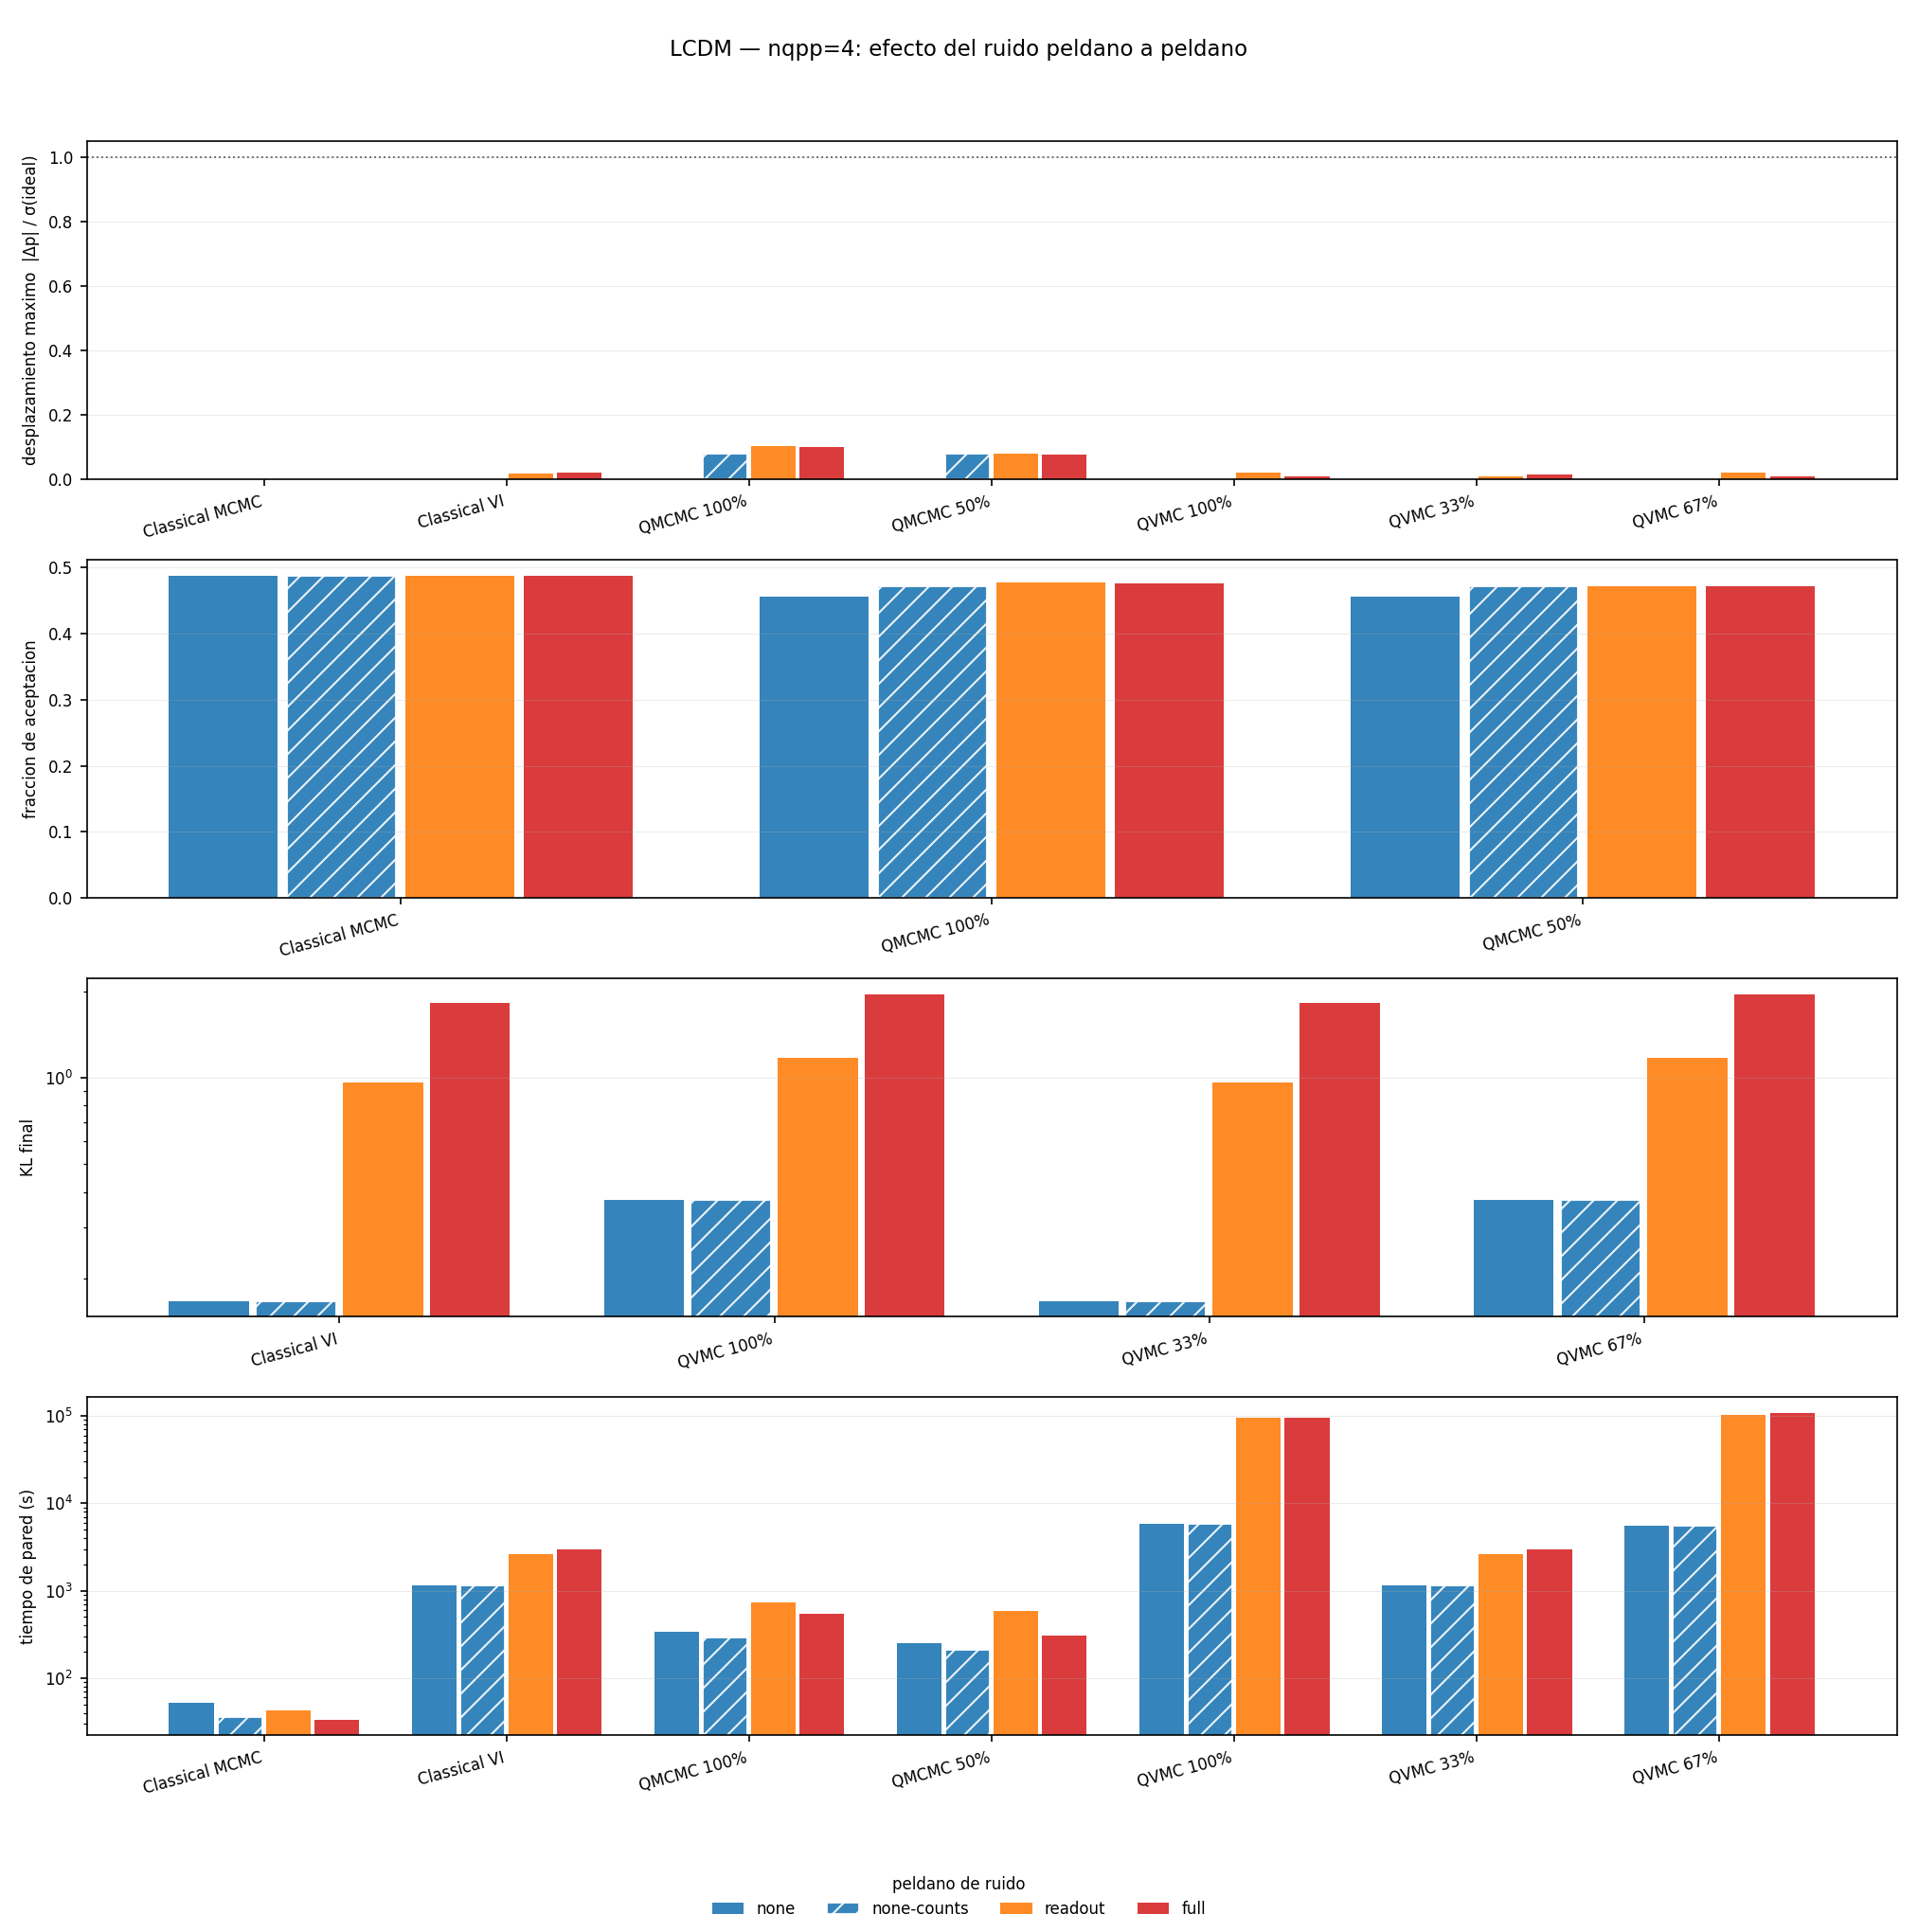
\includegraphics[width=\textwidth]{figs/ejemplo_ruido_fijo.png}
\caption{Figura tipo 3: $\Lambda$CDM a \texttt{nqpp}$=4$, los cuatro
peldaños de ruido lado a lado. De arriba a abajo: desplazamiento (todo
pegado al cero), aceptación (plana), KL (sube con el ruido, escala log) y
tiempo (sube mucho más, escala log). La lectura de conjunto es la conclusión
del eje: \emph{el ruido cuesta tiempo y empeora los diagnósticos internos, y
en la mayoría de las celdas --- ésta incluida --- deja los parámetros donde
estaban}. Las barras rayadas son \texttt{none-counts}.}
\end{figure}

% ---------------------------------------------------------------------
\subsection{Qué buscar al mirarlas}

\begin{enumerate}[leftmargin=1.6em]
  \item \textbf{En el panel de desplazamiento:} ¿alguna barra o punto pasa la
    línea de $1$? Si no, en esa celda el ruido no afecta la ciencia. Y si
    pasa, hay que decir cuál y por qué: las que cruzan son pocas, son
    siempre los peldaños más ruidosos en la rejilla más gruesa, y se
    reproducen en las dos máquinas.
  \item \textbf{En las figuras tipo 1 y 2:} ¿las curvas ruidosas se separan
    de la ideal al crecer el eje $x$? Si se separan, el método se degrada
    con el tamaño del registro, que es una limitación distinta y peor.
  \item \textbf{En el panel de tiempo:} dónde está el salto. En los datos
    actuales el salto está entre el peldaño del $67\%$ y el del $100\%$
    del QVMC, y entre el $67\%$ y el $100\%$ del QGA --- en los dos
    casos, al encender el componente que usa el circuito más ancho.
  \item \textbf{Huecos:} un peldaño que aparece en un panel y no en otro
    quiere decir que esa métrica no aplica a ese método (aceptación en el
    variacional, KL en el genético), no que salga cero.
\end{enumerate}

% =====================================================================
\section{Trabajo relacionado: qué es nuestro y qué no}\label{sec:relacionado}

Hay dos artículos que se llaman «QMCMC» y no son lo mismo. Confundirlos es
la manera más fácil de que a uno le reclamen en una revisión.

\begin{center}
\small
\begin{tabular}{@{}p{3.1cm}p{4.6cm}p{4.6cm}@{}}
\toprule
& \textbf{Layden et al.\ 2023} & \textbf{Sarracino et al.\ 2025 / este trabajo} \\
\midrule
Qué se muestrea
  & configuraciones de espines de un Ising
  & parámetros cosmológicos \\
\addlinespace
Qué son los qubits
  & \textbf{los espines}: el registro \emph{es} el espacio de estados de
    la cadena
  & un generador de aleatoriedad, separado del espacio de parámetros \\
\addlinespace
¿El circuito conoce la distribución objetivo?
  & \textbf{Sí}. La evolución cuántica codifica el Hamiltoniano de Ising
  & \textbf{No}. Los ángulos son aleatorios; el circuito nunca vio la
    posterior \\
\addlinespace
¿Puede haber aceleración?
  & Sí, y la reportan (menos iteraciones que alternativas clásicas)
  & \textbf{No hay mecanismo por el cual pudiera haberla} \\
\addlinespace
Qubits contra tamaño
  & crece con el número de espines del problema
  & crece con $d$ (parámetros), no con los datos \\
\bottomrule
\end{tabular}
\end{center}

\paragraph{Por qué importa, en una frase.} Una propuesta que no sabe dónde
está la posterior no tiene cómo llegar a ella más rápido; lo único que
aporta es una forma distinta de aleatoriedad. Eso explica, sin necesidad de
ninguna otra hipótesis, por qué la razón de ESS medida entre la propuesta
cuántica y la clásica es $\approx 0.95$ y no $> 1$.

Es también la respuesta a la pregunta que un árbitro hará primero:
\emph{¿por qué ustedes no obtienen la aceleración de Layden?} Conviene
además citar la cota de Orfi \& Sels (PRA 110, 052414, 2024), que acota esa
aceleración: usar el resultado de Layden sin la crítica es una omisión
fácil de señalar.

% ---------------------------------------------------------------------
\subsection{Diferencias concretas con Sarracino et al.}

La estructura del circuito de propuesta es la misma (sección 3.1). Difieren
cuatro cosas, y las cuatro hay que declararlas.

\paragraph{1. Cuántos qubits.} Ellos usan $n=\log_2 d$ y aprovechan las
$2^n = d$ amplitudes. Nosotros usamos $n=\max(2,d)$ y tomamos las primeras
$d$ de $2^d$.

\begin{center}
\small
\begin{tabular}{lrrrrr}
\toprule
modelo & $d$ & qubits (ellos) & amplitudes & qubits (nuestros) & amplitudes \\
\midrule
$\Lambda$CDM       & 2 & 1 & 2 de 2 & 2 & 2 de 4 \\
CPL                & 4 & 2 & 4 de 4 & 4 & 4 de 16 \\
Ackley (su prueba) & 8 & 3 & 8 de 8 & 8 & 8 de 256 \\
\bottomrule
\end{tabular}
\end{center}

\noindent
Siempre se cumple $\sum_x |\psi_x|^2 = 1$. Con su esquema las $d$
componentes quedan fuertemente acopladas: si una es grande, las otras
tienen que ser pequeñas. Con el nuestro la restricción se reparte entre
muchas más amplitudes y las $d$ que se usan salen casi independientes. Es
una ventaja real del nuestro, pero \textbf{cuesta exponencialmente más
qubits}, y su escalamiento es mejor. El intercambio hay que justificarlo,
no omitirlo.

\paragraph{2. Qué hace la parte imaginaria.} Ellos:
$s = i\cdot\mathrm{Re}(v)\cdot f(\mathrm{Im}\,v)$, con $f$ una función
escalón que \emph{multiplica o divide} el tamaño de paso. Nosotros:
$\delta = \mathrm{Re}(\psi)\cdot\mathrm{sign}(\mathrm{Im}\,\psi)$.

Con una componente $\mathrm{Re}=0.3$, $\mathrm{Im}=-0.1$: el nuestro da
$\delta = -0.3$ (misma magnitud, cambia la \emph{dirección}); el de ellos
mantiene el signo y divide el paso, dando algo como $+0.15$ (cambia la
\emph{distancia}). Mismos ingredientes, uso opuesto, y dos distribuciones
de propuesta distintas.

\paragraph{3. Cómo se fija la escala.} El desplazamiento crudo tiene
$\sigma \approx 0.35$ y se renormaliza a $\sigma$ unitaria, de modo que sea
un reemplazo directo del $\mathcal{N}(0,1)$ clásico. Ellos ajustan a mano
un «initial step size», y de hecho listan automatizarlo como mejora
pendiente. Aquí la comparación clásico-cuántico queda a escala igualada sin
intervención.

\paragraph{4. Contra qué se compara.} Ellos usan \texttt{emcee}, que --- y
lo dicen --- «uses a different sampling method»: comparan dos algoritmos
distintos a la vez, así que la diferencia observada mezcla el efecto de la
propuesta con el del muestreador. Nosotros comparamos contra el
\textbf{mismo} núcleo de Metropolis--Hastings con un solo componente
cambiado, compartiendo estructura de transición, escala de paso y flujo de
números aleatorios. Ésta es la diferencia metodológica más importante y es
lo que convierte la comparación en un experimento controlado.

Se suma el criterio de convergencia: ellos piden $R-1 < 0.05$ más $\tau$;
aquí se usa $\hat{R}$ split rank-normalizado $< 1.01$ (Vehtari et al.\
2021), bastante más estricto.

\clearpage
% =====================================================================
\section{De la cadena a la barra de error}
% =====================================================================

Todo lo anterior explica cómo se produce \emph{un} punto: un paso de la
cadena, un valor de $\Omega_m$ y $H_0$. Falta el paso que convierte miles de
esos puntos en el resultado que uno escribe en la tesis:

\begin{center}
  $\Omega_m = 0.2772 \pm 0.0103$
\end{center}

\noindent
La respuesta corta es que \textbf{no hay ninguna fórmula de propagación de
errores}. La barra no se calcula: se \emph{mide} sobre la lista de puntos que
la cadena fue anotando. Esta sección hace esa medición con números reales, con
el código \texttt{docs/circuitos/barras\_de\_error.py} (su salida está en
\texttt{barras\_salida.txt}).

% ---------------------------------------------------------------------
\subsection{La lista de puntos \emph{es} la respuesta}

El teorema que sostiene todo Metropolis--Hastings dice: si la cadena corre lo
suficiente, \textbf{la frecuencia con la que visita cada región del espacio de
parámetros es proporcional a la probabilidad posterior de esa región}. No
converge a un número: converge a una \emph{distribución de visitas}.

Entonces, al terminar, uno tiene una lista de $N$ puntos ---en el ejemplo, 4
cadenas $\times$ 3000 pasos--- y esa lista \emph{ya es} una muestra de la
posterior. Hacer un histograma de la columna de $\Omega_m$ no es una
aproximación a la posterior: es la posterior, tal como la cadena la conoce
(figura~\ref{fig:barras}, panel b).

\begin{figure}[H]
\centering
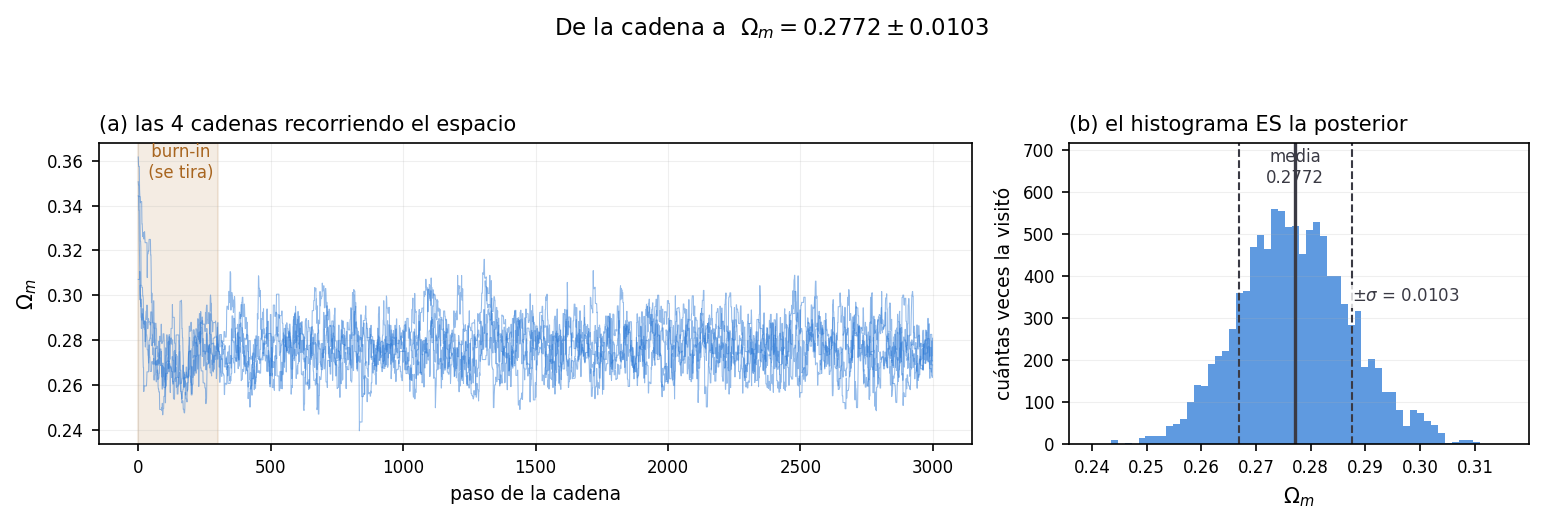
\includegraphics[width=\textwidth]{figs/barras_de_error.png}
\caption{Izquierda: las cuatro cadenas. Arrancan lejos, caen a la zona buena
en los primeros $\sim 200$ pasos (el transitorio sombreado, que se tira) y
después se quedan oscilando alrededor del mismo valor. Derecha: el histograma
de todos los puntos posteriores al transitorio. La línea sólida es la media;
las punteadas, $\pm$ una desviación estándar. Ese ancho \emph{es} la barra de
error.}
\label{fig:barras}
\end{figure}

% ---------------------------------------------------------------------
\subsection{Los puntos repetidos son los rechazos}

Esto es lo que más confunde, y es la pieza central. Cuando un paso se
\emph{rechaza}, la cadena \textbf{no se salta el renglón}: vuelve a anotar el
punto en el que ya estaba. Los diez primeros pasos de una cadena real:

\begin{center}
\small
\begin{tabular}{rrrl}
\toprule
paso & $\Omega_m$ & $H_0$ & qué pasó \\
\midrule
0 & 0.35061 & 65.130 & se movió (aceptó) \\
1 & 0.34917 & 64.640 & se movió (aceptó) \\
2 & 0.34917 & 64.640 & \Cl{se quedó (rechazó)} \\
3 & 0.34398 & 64.807 & se movió (aceptó) \\
4 & 0.34398 & 64.807 & \Cl{se quedó (rechazó)} \\
5 & 0.34398 & 64.807 & \Cl{se quedó (rechazó)} \\
6 & 0.34398 & 64.807 & \Cl{se quedó (rechazó)} \\
7 & 0.34398 & 64.807 & \Cl{se quedó (rechazó)} \\
8 & 0.34120 & 65.338 & se movió (aceptó) \\
9 & 0.34177 & 64.957 & se movió (aceptó) \\
\bottomrule
\end{tabular}
\end{center}

\noindent
El punto $(0.34398,\,64.807)$ aparece \textbf{cinco veces} en la lista. En el
histograma cuenta cinco veces. Ése es todo el mecanismo: \emph{un punto bueno
que rechaza muchas propuestas se queda anotado muchas veces y su barra del
histograma crece; un punto malo se abandona rápido y casi no aparece.} Es así
como el peso de cada región termina siendo proporcional a su probabilidad, sin
que nadie calcule nunca una integral.

La contabilidad cierra exactamente:

\begin{center}
\small
\begin{tabular}{lr}
\toprule
puntos repetidos & $6291 / 11996 = 0.5244$ \\
$1 - \text{aceptación}$ & $1 - 0.4755 = 0.5245$ \\
\bottomrule
\end{tabular}
\end{center}

\noindent
Son la misma cantidad por definición. Por eso la columna
\texttt{acceptance} del CSV es un diagnóstico y no un resultado: dice qué
fracción de la lista son repeticiones.

\paragraph{Y aquí vuelve a aparecer el circuito~2.} Quién se repite y quién no
lo decide, paso por paso, la moneda de la aceptación. En las celdas con
aceptación cuántica esa moneda es el circuito de un qubit de la
sección~\ref{sec:aceptacion}. Que ese circuito sea \Fi{fiel} ---que reproduzca
$\min(1, e^{\Delta})$ de forma exacta--- es justamente lo que garantiza que el
histograma salga idéntico al clásico, y por lo tanto que la barra de error
salga idéntica. La prueba de fidelidad no es un tecnicismo: es lo que permite
afirmar que la barra de error reportada sigue siendo correcta.

% ---------------------------------------------------------------------
\subsection{La cuenta, y dónde está en el CSV}

Con la lista ya construida, el cálculo es de primaria:

\begin{equation}
  \bar{\Omega}_m = \frac{1}{N}\sum_{i=1}^{N} \Omega_m^{(i)},
  \qquad
  \sigma_{\Omega_m} = \sqrt{\frac{1}{N-1}\sum_{i=1}^{N}
    \bigl(\Omega_m^{(i)} - \bar{\Omega}_m\bigr)^2}.
\end{equation}

\noindent
Nada más. Y esas dos cantidades son, literalmente, las columnas
\texttt{Om\_mean} y \texttt{Om\_std} del archivo de resultados
(\texttt{resultados\_config.csv}). La corrida de esta sección contra lo que la
campaña reportó para la misma celda ($\Lambda$CDM, \texttt{nqpp}$=3$,
\texttt{noise=none}):

\begin{center}
\small
\begin{tabular}{lrr}
\toprule
& esta corrida & la campaña \\
\midrule
$\Omega_m$ & $0.277152 \pm 0.010301$ & $0.276444 \pm 0.010486$ \\
$H_0$      & $69.5490 \pm 0.7946$    & $69.5949 \pm 0.8007$ \\
\bottomrule
\end{tabular}
\end{center}

\noindent
No son idénticos ---son semillas distintas y longitudes distintas--- pero son
la misma cantidad calculada de la misma manera. Que coincidan a este nivel es
en sí mismo una comprobación.

\paragraph{Percentiles, cuando la posterior no es simétrica.} La media y la
desviación estándar suponen implícitamente que la distribución es más o menos
una campana. Cuando no lo es, se reportan los percentiles 16/50/84, que dan
una barra asimétrica. Aquí:

\begin{center}
\small
$\Omega_m$: $\;0.26715 \;/\; 0.27674 \;/\; 0.28740
  \;\Longrightarrow\; 0.2767^{+0.0107}_{-0.0096}$
\end{center}

\noindent
Comparado con $0.2772 \pm 0.0103$, la asimetría es de un $10\%$ del ancho: la
posterior de $\Lambda$CDM con estos datos es casi gaussiana y las dos formas
de reportar dicen lo mismo. En CPL, con $w_a$ mal restringido, no lo son, y
ahí conviene dar percentiles.

% ---------------------------------------------------------------------
\subsection{Las tres condiciones para que la barra valga}

La barra es correcta sólo si se cumplen tres cosas. Las tres son
verificables y las tres están medidas en la campaña.

\paragraph{(a) El transitorio se tira.} Las cadenas arrancan en un punto
arbitrario ---en la figura, cerca de $\Omega_m = 0.35$--- y tardan unos
cientos de pasos en llegar a la zona de probabilidad alta. Esos puntos
iniciales no son muestras de la posterior: son el viaje hacia ella. Si se
dejan, inflan el ancho:

\begin{center}
\small
\begin{tabular}{lr}
\toprule
sin tirar el burn-in & $\Omega_m = 0.277130 \pm 0.011292$ \\
tirándolo (300 pasos) & $\Omega_m = 0.277152 \pm 0.010301$ \\
\bottomrule
\end{tabular}
\end{center}

\noindent
La media casi no cambia; la $\sigma$ baja un $9\%$. El transitorio mete puntos
lejanos que el estimador de dispersión lee como anchura real de la posterior
cuando en realidad son el arranque.

\paragraph{(b) Las cadenas coinciden entre sí: $\hat{R} < 1.01$.} $\hat{R}$
compara la dispersión \emph{dentro} de cada cadena con la dispersión
\emph{entre} las cuatro. Si las cuatro exploraron la misma distribución, las
dos dispersiones tienen que ser iguales y $\hat{R} \to 1$. Si una se quedó
atorada en otra región, la dispersión entre cadenas es mayor y $\hat{R}$ sube.
Medido aquí: $\hat{R} = 1.00035$. El criterio de la campaña es el $\hat{R}$
split rank-normalizado de Vehtari et al.\ (2021) con umbral $1.01$.

Un $\hat{R}$ malo invalida la barra por completo: significa que ni siquiera se
sabe si la lista es una muestra de la posterior.

\paragraph{(c) Hay suficientes muestras \emph{independientes}: el ESS.} Aquí
está el punto fino. Los puntos de una cadena \textbf{no son independientes}:
el paso $t+1$ sale del paso $t$ con un desplazamiento chico, y además, como se
vio arriba, la mitad son copias literales del anterior. Una lista de 10\,800
puntos de una cadena no vale lo mismo que 10\,800 sorteos independientes.

El \emph{effective sample size} traduce la lista a su equivalente
independiente:

\begin{equation}
  \mathrm{ESS} = \frac{N}{1 + 2\sum_{k\ge 1}\rho_k},
\end{equation}

\noindent
con $\rho_k$ la autocorrelación a distancia $k$. Medido aquí:
$\mathrm{ESS} = 453$ de $N = 10\,800$, es decir que \textbf{hacen falta unos
24 pasos de cadena para ganar una muestra independiente}.

Esto cambia una cosa concreta, y es un error común equivocarla. La
\textbf{anchura de la posterior} es $\sigma = 0.0103$ y no depende del ESS: es
una propiedad de los datos y del modelo, no de cuánto se corrió. Lo que sí
depende del ESS es el \textbf{error de la media}, o sea qué tan bien está
determinado el centro:

\begin{center}
\small
\begin{tabular}{lr}
\toprule
correcto: $\sigma / \sqrt{\mathrm{ESS}}$ & $0.000484$ \\
incorrecto: $\sigma / \sqrt{N}$ & $0.000099$ \\
\bottomrule
\end{tabular}
\end{center}

\noindent
Usar $\sqrt{N}$ en lugar de $\sqrt{\mathrm{ESS}}$ hace creer que el centro está
casi cinco veces mejor determinado de lo que está. Éste es el único lugar del
análisis donde el ESS entra directamente en un número reportado.

% ---------------------------------------------------------------------
\subsection{Por qué el ESS es la métrica para comparar muestreadores}

De lo anterior sale, sin ninguna hipótesis extra, la métrica con la que se
comparan QMCMC y el MCMC clásico. Los dos llegan a la misma barra de error
---deben llegar, y eso es la prueba de fidelidad---, así que el resultado no
los distingue. Lo que los distingue es \textbf{cuántas muestras independientes
produjeron por paso}, y eso es exactamente el ESS.

\begin{center}
\small
\begin{tabular}{lrrr}
\toprule
& ESS & aceptación & tiempo (s) \\
\midrule
Classical MCMC & 6872 & 0.4873 & 92.5 \\
QMCMC 50\% & 6956 & 0.4560 & 354.3 \\
QMCMC 100\% & 6956 & 0.4560 & 437.0 \\
\bottomrule
\end{tabular}
\end{center}

\noindent
($\Lambda$CDM, \texttt{nqpp}$=3$, sin ruido.) En esta celda la propuesta
cuántica sale ligeramente arriba; sobre los cinco modelos, la razón mediana de
ESS es $0.948$ y sólo 2 de 5 quedan a favor. La conclusión honesta es
\textbf{empate}, y la sección~\ref{sec:relacionado} explica por qué era lo esperado: una propuesta
que no sabe dónde está la posterior no tiene mecanismo para llegar más rápido.

% ---------------------------------------------------------------------
\subsection{Por qué el QVMC reporta una barra más chica, y por qué eso es malo}

El variacional produce su $\sigma$ de otra manera: no por muestreo, sino
evaluando la distribución ajustada sobre la rejilla. Y sale sistemáticamente
más angosta. Las razones contra el MCMC clásico, sobre toda la campaña:

\begin{center}
\small
\begin{tabular}{lrrrrr}
\toprule
método & $\Omega_m$ & $H_0$ & $w$ & $w_0$ & $w_a$ \\
\midrule
QMCMC 50\% / 100\% & 0.994 & 0.998 & 1.018 & 0.991 & 0.903 \\
Classical VI       & 0.803 & 0.807 & 0.813 & 0.826 & 0.801 \\
QVMC 33\%          & 0.812 & 0.806 & 0.815 & 0.822 & 0.808 \\
QVMC 67\% / 100\%  & 0.675 & 0.703 & 0.551 & 0.857 & 0.534 \\
\bottomrule
\end{tabular}
\end{center}

\noindent
\textbf{Reportar menos incertidumbre de la que hay no es una mejora: es un
sesgo.} La causa es conocida y no es un error de implementación: el
variacional minimiza $\mathrm{KL}(q \| p)$, que castiga muchísimo poner
probabilidad donde la posterior no tiene y casi no castiga dejar de ponerla
donde sí hay. El óptimo de esa asimetría es una distribución que se mete en el
modo y se encoge. Es el comportamiento estándar de la inferencia variacional,
visible ya en la fila \emph{Classical VI}, donde no hay nada cuántico.

Lo que sí aporta el marco de ablación es medir cómo escala con los peldaños:
el sesgo pasa de $0.80$ con un componente cuántico a $0.53$--$0.86$ con dos o
tres. Es decir, \textbf{los componentes cuánticos del QVMC empeoran un sesgo
que ya existía}. Eso es un resultado reportable y va con su figura
(\texttt{incertidumbre\_reportada.png}).

\paragraph{Y las columnas \texttt{*\_std} del genético no son barras de error.}
Un algoritmo genético converge a un \emph{punto}, no a una distribución. Su
\texttt{Om\_std} mide cuánto se encogió la población alrededor del mejor
individuo, que es un diagnóstico de convergencia del optimizador. Sus valores
($0.07$--$0.18$ veces la $\sigma$ del MCMC) no significan que el genético
determine los parámetros cinco veces mejor: significan que la población se
apretó. Ponerlos en la misma figura que las $\sigma$ de los muestreadores es
un error, y por eso \texttt{comparar\_algoritmos.py} los separa en otra sección
y los imprime con un aviso.

% ---------------------------------------------------------------------
\subsection{Resumen de la sección}

\begin{enumerate}[leftmargin=1.6em]
  \item La cadena visita cada región en proporción a su probabilidad, así que
    la lista de puntos \emph{es} la posterior.
  \item Los rechazos repiten el punto anterior; esa repetición es el mecanismo
    que le da peso a lo probable. Su fracción es $1 -$ aceptación.
  \item La barra de error es la desviación estándar de esa lista ---las
    columnas \texttt{*\_std} del CSV---, no una propagación de errores.
  \item Vale si se tiró el transitorio, si $\hat{R} < 1.01$ y si el ESS es
    suficiente. El ESS no cambia la anchura de la posterior; cambia el error
    de su centro, por $\sqrt{\mathrm{ESS}}$ y no por $\sqrt{N}$.
  \item El ESS es la métrica de comparación entre muestreadores precisamente
    porque la barra de error \emph{no} los distingue: llegan a la misma, y
    deben hacerlo.
  \item Una $\sigma$ más chica no es un método mejor. En el QVMC es sesgo de
    la KL, y empeora al subir los peldaños.
\end{enumerate}

\clearpage
\section{Resumen}
% =====================================================================

\begin{center}
\small
\begin{tabular}{llll}
\toprule
\textbf{\#} & \textbf{Circuito} & \textbf{Qubits} & \textbf{Clase} \\
\midrule
1 & QMCMC / propuesta        & $d$            & \Cu{algorítmico} \\
2 & QMCMC / aceptación       & $1$            & \Fi{fiel (probado)} \\
3 & QVMC / ansatz            & $d\cdot n_{qpp}$ & \Fi{fiel} al muestrear \\
3bis & QVMC / gradiente      & ídem, $1+2n_\varphi$ circuitos & \Cu{algorítmico} \\
4 & QVMC / normalización     & $n+1$          & \Fi{fiel por construcción} \\
5 & QGA / inicialización     & $d\cdot n_b$   & \Cu{algorítmico} \\
6 & QGA / mutación           & $n_b$          & \Cu{algorítmico} \\
7 & QGA / cruce              & $2 n_b$        & \Cu{algorítmico} \\
\bottomrule
\end{tabular}
\end{center}

\medskip
\noindent
Tres cosas que conviene tener presentes al escribir sobre esto:

\begin{enumerate}[leftmargin=1.6em]
  \item \textbf{La prueba fuerte del marco es el circuito 2.} Es el único
    componente donde la igualdad cuántico\,=\,clásico es un teorema de una
    línea y una verificación numérica exacta, no una consecuencia de cómo
    está escrito el código.
  \item \textbf{El circuito 3 tiene un techo estructural.} $7n$ ángulos
    contra $2^n-1$ grados de libertad. La KL no baja a cero y no debería
    esperarse que lo haga.
  \item \textbf{El circuito 7 es el que fija el costo del eje de ruido.}
    $2n_b$ qubits más matriz de densidad es lo que hace inviable el peldaño
    del $100\%$ ruidoso a partir de $n_b = 6$.
\end{enumerate}

\end{document}
